\documentclass[a4paper,11pt]{article}

\usepackage[utf8]{inputenc} % allow utf-8 input
\usepackage[T1]{fontenc}    % use 8-bit T1 fonts
\usepackage{hyperref}       % hyperlinks
\usepackage{url}            % simple URL typesetting
\usepackage{booktabs}       % professional-quality tables
\usepackage{amsfonts}       % blackboard math symbols
%\usepackage{nicefrac}       % compact symbols for 1/2, etc.
\usepackage{microtype}      % microtypography

\usepackage{amssymb,amsmath}
%\usepackage{graphicx}
%\usepackage{babel}
%\usepackage[veryoldstyle,largesmallcaps]{kpfonts}
\usepackage{lmodern}
\usepackage{parskip}
\usepackage{capt-of}
\usepackage{amsmath} % pour \ddots
\usepackage{xfp}
 \usepackage{xcolor}
 \usepackage{graphicx}
 \usepackage{multirow}
\usepackage{array}
\usepackage{tikz}
\usepackage{pgfplots}
\usepackage[ruled, french]{algorithm2e}
\usepackage{pgfplotstable}
\pgfplotsset{compat = newest}
\usepackage[french,english]{babel}
\usepackage{float}
%\graphicspath{ {./images/} }
\usepackage{mathtools}
\usepackage[margin=1in]{geometry} % Ajuste les marges
\usepackage{lipsum} % Pour générer du texte factice
\usepackage{geometry}
\geometry{left=2.5cm,right=2.5cm,bottom=3cm, top=3cm}
\usepackage{fancyhdr}
\pagestyle{fancy}
\usepackage{caption}

\usetikzlibrary{shapes, arrows}

\renewcommand{\headrulewidth}{0pt}
\fancyhead[L]{
\includegraphics[width=2cm]{images/ece.png}}
\fancyhead[R]{ING{3} Groupe{3}}
\definecolor{ece}{RGB}{0, 122, 123}

\usepackage{listings}
\usepackage{xcolor}

\usepackage[most]{tcolorbox}

\newtcolorbox{citationbox}{
  enhanced,
  colback=white,           % Fond blanc
  colframe=white,          % Pas de cadre
  boxrule=0pt,             % Épaisseur du cadre (ici désactivé)
  borderline west={2pt}{0pt}{gray}, % Ligne verticale à gauche
  left=10pt,               % Marge intérieure à gauche
  right=10pt,              % Marge intérieure à droite
  top=5pt,                 % Marge intérieure en haut
  bottom=5pt               % Marge intérieure en bas
}

\definecolor{codegreen}{rgb}{0,0.6,0}
\definecolor{codegray}{rgb}{0.5,0.5,0.5}
\definecolor{codepurple}{rgb}{0.58,0,0.82}
\definecolor{backcolour}{rgb}{0.95,0.95,0.92}

\lstdefinestyle{mystyle}{
    backgroundcolor=\color{backcolour},   
    commentstyle=\color{codegreen},
    keywordstyle=\color{magenta},
    numberstyle=\tiny\color{codegray},
    stringstyle=\color{codepurple},
    basicstyle=\ttfamily\footnotesize,
    breakatwhitespace=false,         
    breaklines=true,                 
    captionpos=b,                    
    keepspaces=true,                 
    numbers=left,                    
    numbersep=5pt,                  
    showspaces=false,                
    showstringspaces=false,
    showtabs=false,                  
    tabsize=2
}

\lstset{style=mystyle}


\begin{document}

\begin{titlepage}
    \noindent
    \begin{center}
        \centering
        
\includegraphics[width=7cm]{images/ece.png} % Remplacez par le chemin de votre logo
    \end{center}
	\vfill
	
	\vspace{1cm}
	\makebox[\linewidth]{\rule{\textwidth}{0.4pt}} % Ligne horizontale supérieure
    
    \centering
    {\Huge Rapport Neural Speech\par}
    
    \makebox[\linewidth]{\rule{\textwidth}{0.4pt}} % Ligne horizontale inférieure
    \vspace{1cm}	
	
    \begin{minipage}[t]{0.45\textwidth}
        \centering
        {\Large Axel Bröns \\ \texttt{\href{mailto:axel.brons@edu.ece.fr}{axel.brons@edu.ece.fr}}}
    \end{minipage}
    \hfill
    \begin{minipage}[t]{0.45\textwidth}
    	\centering
        {\Large Valentin Kocijancic \\ \texttt{\href{mailto:valentin.kocijancic@edu.ece.fr}{valentin.kocijancic@edu.ece.fr}}}
    \end{minipage}   
    \vfill
    \begin{minipage}[t]{0.45\textwidth}
        \centering
        {\Large Hugo Rivière \\ \texttt{\href{mailto:hugo.riviere@edu.ece.fr}{hugo.riviere@edu.ece.fr}}}
    \end{minipage}
    \hfill
    \begin{minipage}[t]{0.45\textwidth}
    	\centering
        {\Large Ethan Petain \\ \texttt{\href{mailto:ethan.petain@edu.ece.fr}{ethan.petain@edu.ece.fr}}}
    \end{minipage}  
    
    
    
    \vfill
    {\large Lyon, le 6 avril 2025\par}
    \vspace{1cm}
    {\normalsize Ce projet est un travail réalisé par des étudiants sans objectif de commercialisation. Nous attestons que ce travail est original, qu’il est le fruit d’un travail commun au groupe et qu’il a été rédigé de manière autonome.\par}
\end{titlepage}

\newpage
\begin{abstract}
Le projet Neural Speech sous le nom de \textit{Couleur Master} vise à développer un système embarqué de reconnaissance vocale capable d'identifier des mots simples, tels que des noms de couleurs, pour faciliter l'apprentissage des enfants ou des personnes en rééducation linguistique. Basé sur une carte Arduino Due, notre solution combine un traitement avancé du signal audio et un réseau de neurones pour analyser et classer les entrées vocales en temps réel. L'utilisation d'algorithmes performant et avancés comme par exemple l'algorithme MFC ont permis de réduire la complexité de la capacité du micro-contrôleur tout en conservant les informations essentielles.

Un réseau de neurones simple mais efficace, entraîné avec TensorFlow, permet une classification robuste des mots enregistrés, avec une précision dépassant 98\%. Le système est intégré dans une boîte autonome alimentée par batterie, comprenant un microphone, des LEDs indicatrices et un bouton de commande. Des fonctionnalités bonus, comme la détection d'erreurs ou l'ajout d'une nouvelle couleur, ont été ajoutées pour améliorer l'expérience utilisateur.

Ce projet démontre avec succès l'application pratique de l'IA embarquée, tout en soulignant les défis liés aux contraintes matérielles. Les résultats obtenus ouvrent des perspectives d'amélioration, notamment avec une détection en temps réel ou alors avec un dataset élargi. Couleur Master illustre ainsi la puissance de l'électronique et de l'informatique combinées pour créer des outils pédagogiques innovants.
\end{abstract}
\newpage
\tableofcontents
\newpage

\section{Objectifs}
Ce document montre notre implication et les détails techniques du projet \textbf{Neural Speech} et atteste de la sincérité de notre travail. Vous pourrez trouver dans ce document les attendus du projet comme l’étude documentaire ou encore les différentes exigences techniques. On rappel que ce document est un travail réalisé par des étudiants sans objectif de commercialisation.
	
\section{Glossaire}
\subsection{Termes}
Nous listons les termes que nous allons fréquemment utiliser dans ce document : 
\begin{table}[H]
\centering
\begin{tabular}{|l|p{10cm}|}
\hline
\textbf{Terme technique} & \textbf{Définition} \\
\hline
Flash ADC & Type de convertisseur qui transforme un signal analogique en valeur numérique \\ 
\hline
Aliasing & Phénomène qui se produit lorsqu’un signal est échantillonné à une fréquence trop faible, il y a repliement de spectre\\
\hline
Down-sampling & Réduction la résolution spatiale ou temporelle du signal \\
\hline
Buffer & Zone de mémoire temporaire utilisée pour stocker des données en transit\\
\hline
Padding & Préserve la dimension des signaux lors du filtrage \\
\hline
Pooling & Technique qui consiste à réduire la taille des données tout en conservant l’information essentielle \\
\hline
Flatten & Opération qui permet de réduire en une dimension une structure de donnée multidimensionnelle \\
\hline
Epochs & Passage complet sur l’ensemble des données d'entraînement\\
\hline
Kernels & Petites matrices utilisées pour l'extraction de caractéristiques à partir de données d'entrée telles que des images \\
\hline
\end{tabular}
\end{table}
			
\subsection{Acronymes} \label{acro}
Le tableau des acronyme est volumineux alors nous l'avons mis en annexe, à la table \ref{table:acro}.
			
\section{L'équipe}
\subsection{Présentation de l’équipe}
L’équipe est composée de 4 étudiants :
\begin{itemize}
\item \textbf{BRONS Axel} : Le technicien, il manie la pratique et la théorie à la perfection. Il a une grande compréhension du cours théorique et une expertise pour la réalisation pratique.
\item \textbf{KOCIJANCIC Valentin} : L’ingénieur, il sait résoudre les problèmes que ce soit au niveau de la maquette qu’au niveau réflexion dans le cours théorique. Au moindre problème, on fait appel à lui. 
\item \textbf{PETAIN Ethan} : L'informaticien, il peut faire n’importe quoi avec un ordinateur. Quand on n’arrive pas trouver la solution d'un problème de code ou d'informatique, on se tourne vers lui. 
\item \textbf{RIVIERE Hugo} : Rédacteur professionnel, il sait bien embellir la situation, de plus il apporte un soutien moral à toute l'équipe.
\end{itemize}
\begin{figure}[H]
\begin{minipage}{0.20\textwidth}
\centering
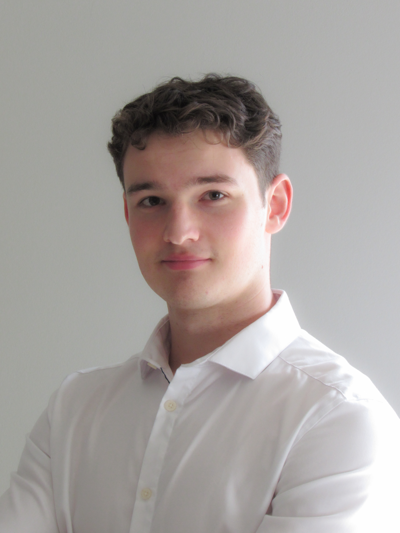
\includegraphics[scale=0.7]{images/axel.png}
\caption*{Axel Bröns}
\end{minipage}
\hfill
\begin{minipage}{0.20\textwidth}
\centering
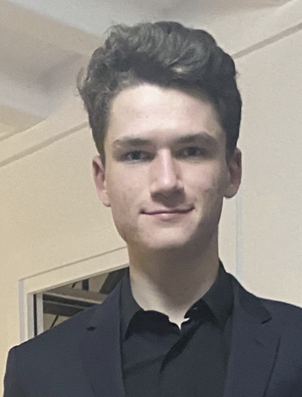
\includegraphics[scale=0.7]{images/valentin.png}
\caption*{Valentin Kocijancic}
\end{minipage}
\hfill
\begin{minipage}{0.20\textwidth}
\centering
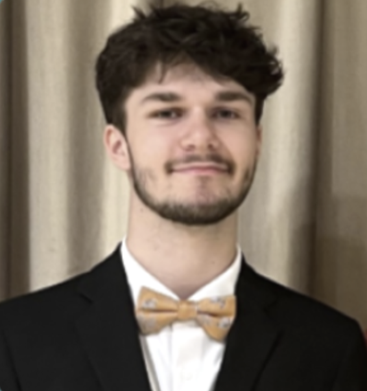
\includegraphics[scale=0.7]{images/ethan.png}
\caption*{Ethan Petain}
\end{minipage}
\hfill
\begin{minipage}{0.20\textwidth}
\centering
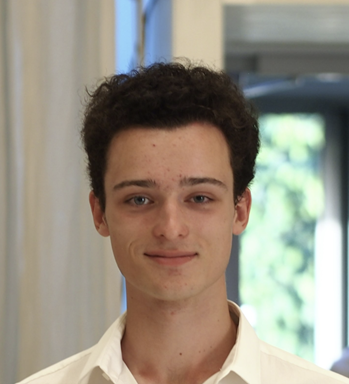
\includegraphics[scale=0.7]{images/hugo.png}
\caption*{Hugo Rivière}
\end{minipage}
\hfill
\end{figure}
			
\subsection{Organisation de l’équipe}
Notre organisation du travail dans l’équipe a été faite de manière très simple et efficace. Nous  nous connaissons bien, ce qui à grandement aidé à trouver un équilibre et une ambiance de travail. Pour ce faire nous avons diviser les tâches entre nous. Hugo contribuer au rapport, Valentin au FS3 et FS4, Ethan au FS5. Axel quand à lui a réaliser l’ensemble des tâches pour ne pas perdre le fil conducteur du projet et pouvoir rassembler les deux parties (IA et traitement du signal) plus efficacement.

\subsection{Diagramme de Gantt}
\begin{figure}[H]
\centering
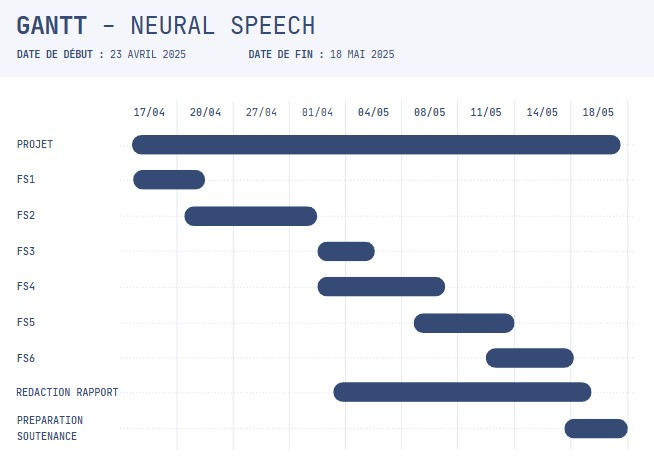
\includegraphics[scale=0.6]{images/gantt2.jpg}
\end{figure}
Le diagramme de Gantt nous a permis de ne pas se perdre dans toutes les exigences techniques du projet et ainsi pouvoir rendre un livrable à temps et fonctionnel.

\section{Contexte et problématique}
\subsection{Contexte}
Pour le projet d'électronique du second semestre de la troisième année du cycle préparatoire, nous avons choisi de faire la différence de trois couleurs. Nous avons convenu que ce projet servirai à aider les enfants pour apprendre les couleurs. Pour ce faire nous pensons pouvoir mettre en place toute les couleurs différentes dans le réseau de neurone. Ce qui serai un outil très utile et ludique pour les enfants. Cela leur permettrai d’apprendre les couleurs mais aussi à prononcer correctement ces mots-là.  En amélioration supplémentaire nous pourrons développer ce concept pour non plus seulement des couleurs mais bien plus de mots utiles pour les petits enfants qui apprennent à parler.  De plus ce projet pourrai être étendu au personne qui veulent apprendre le français, ou qui doivent suivre une rééducation linguistique.

\subsection{Problématique}
		
Ce projet répond à la problématique suivante :
\begin{citationbox}
Comment faciliter l'apprentissage des couleurs pour les personnes à bas âge ou sous rééducation linguistique ?
\end{citationbox}
			
\subsection{Spécifications techniques}
Les attendus techniques sont de faire un projet de reconnaissance vocale basé sur une IA embarquée. Pour ce faire nous devrons réussir à numériser un signal audio, puis à le traiter numériquement pour pouvoir le passer dans un réseau de neurone. Ce projet doit être fait impérativement sur la carte Arduino Due pour que le système puisse être de l’embarqué.
			
\section{Conception}
\subsection{Architecture fonctionnelle}
L'architecture fonctionnelle suit les fonctions suivantes :
\begin{itemize}
	\item Enregistrer un mot à l'aide d'un microphone
	\item Transformer l'audio pour avoir des valeurs
	\item Convertir ces valeurs en données exploitables
	\item Reconnaître le mot
	\item Afficher la lumière correspondant au mot dit
\end{itemize}
			
\subsection{Architecture matérielle}
Le matériel utilisé lors de ce projet est la carte Arduino DUE (\href{https://docs.arduino.cc/resources/datasheets/A000062-datasheet.pdf}{Datasheet de l'Arduino Due}), un microphone Arduino (\href{https://www.analog.com/media/en/technical-documentation/data-sheets/max9814.pdf}{Datasheet du MAX9814}), d'un bouton poussoir, de LED rouges, verts, bleus et jaune, ainsi qu'un câble de connexion pour connecter la carte à un ordinateur. Pour les validations des différentes parties nous avons aussi utilisé du matériel en plus comme un oscilloscope et un GBF. Nous avons aussi utilisé une boîte en carton pour réaliser notre maquette ainsi qu'une batterie externe que nous connecterons à la carte pour que le système soit totalement indépendant et 100\% embarqué. Voici le schéma de notre circuit sur KiCad :
\begin{figure}[H]
\centering
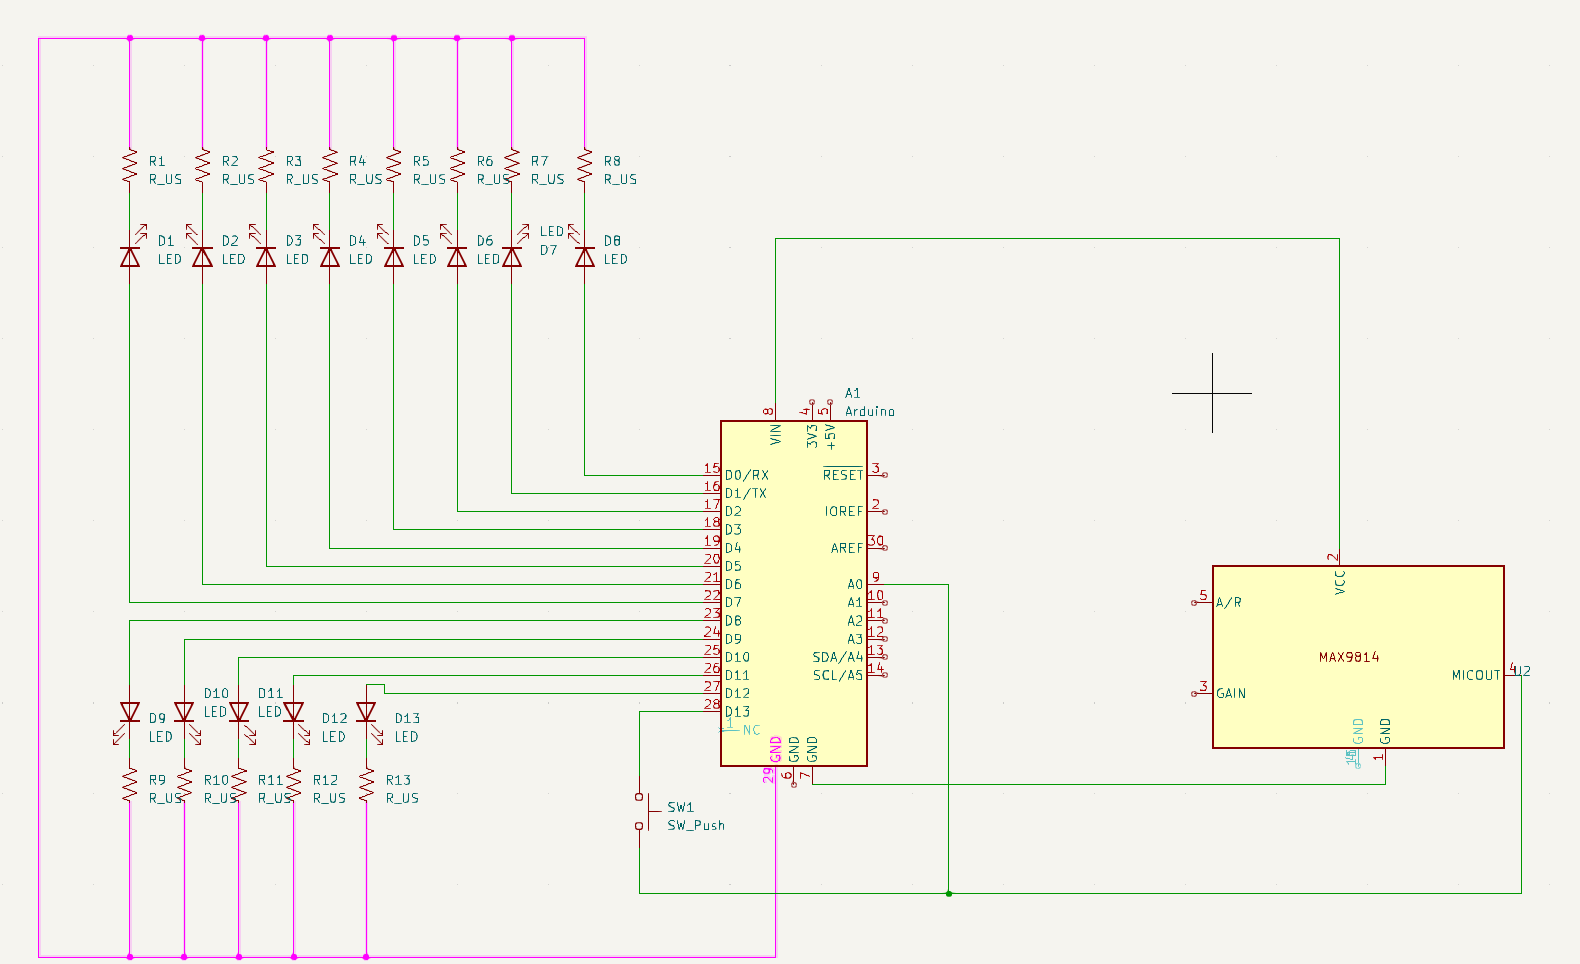
\includegraphics[scale=0.35]{images/kicad.png}
\caption{Schéma électronique \textbf{KiCad} de notre montage final}
\end{figure}
			
\subsection{Architecture logicielle}
Nous avons utilisé plusieurs pour mettre à bien ce projet, en effet, nous avons mis en place un code permettant d'enregistrer les différentes données d'entrainement en appliquant le traitement du signal adéquate, ensuite nous avons un code \texttt{Python} pour entraîner notre réseau de neurones et pour finir nous avons un dernier code \texttt{C++} qui rassemble ces deux parties et qui concerne la prédictions avec les valeurs qu'on enregistre en direct via le microphone tout en faisant le traitement du signal comme dans le premier code. L'algorigramme du code pour enregistrer les données est disponible à la figure \ref{fig:algo_enregistrement}, l'algorigramme pour notre code Python est quant à lui disponible à la figure \ref{fig:algo_cnn} et pour finir l'algorigramme de prédictions est disponible à la figure \ref{fig:prediction}.
	
\section{Développement}
			
\subsection{Traitement du signal} \label{traitement}

\subsubsection{Numériser le signal audio} \label{numeriser}

Le but de cette partie est de passer notre signal à 32KHz et par la suite appliquer un filtre numérique. D'abord, nous devons absolument avoir l’Arduino Due en mode d’interruption sur timer pour pouvoir avoir un échantillonnage fixe et précis. Nous voulons avoir un signal avec une fréquence d'acquisition de 32 MHz. Pour cela, nous voulons trouver la valeur théorique du registre $RC$. Pour cela, nous utilisons le \texttt{Timer\_Clock1}, ainsi on peut calculer la valeur de $RC$ grâce à la formule suivante : 
\begin{equation} \label{eq:rc}
	RC = \frac{MCK}{PF} = \frac{84000000}{2 \times 32000} \approx 1312
\end{equation}
Avec $MCK = 84 \text{MHz}$, la valeur de la Master Clock, $F$ la fréquence voulue et $P$ le prescaler utilisé (dans notre cas notre prescaler vaut 2, parce qu'on utilise la \texttt{Clock1}). La raison de pourquoi nous voulons 32 KHz, est lié à une règle de base en traitement du signal : le théorème de \textbf{Nyquist-Shannon}. Ce théorème nous dit que pour représenter un signal sans perte, il faut échantillonner à au moins 2 fois la fréquence maximale qu'on veut capter. Ainsi, si on veut capter toutes les fréquences jusqu’à 16 kHz, il faut au moins 32 kHz d’échantillonnage. Nous faisons alors un compromis entre la qualité du signal et charge de traitement. En effet, nous pourrons laisser à 44KHz, mais nous aurons une plus grande plage de valeurs coûteuse pour notre Arduino Due. Ainsi, nous décidons de choisir 32KHz puisque la fréquence seuil qu'un humain peut entendre est de 20KHz. Ainsi, ce théorème peut se représenter par la formule suivante : 
\begin{equation}
	f_s \geq 2f_m
\end{equation}
Avec $f_s$ la fréquence d'échantillonnage et $f_m$ la fréquence maximale du signal. Dans notre cas, $f_s = 32000$ et $f_s \leq 16000$. 

\subsubsection{Filtre RIF} \label{rif}

Après avoir échantillonné notre signal à 32KHz nous devons filtrer les fréquences supérieurs à 4KHz et les atténuer d'au moins 30dB. Nous devons les filtrer pour éviter l'effet de repliement (aliasing en anglais) ce qui déformerait notre enregistrement audio. Nous devons appliquer un filtre, pour rappel, un filtre est un système qui modifie certaines composantes d’un signal, généralement en fréquence. Il peut atténuer le bruit, supprimer les hautes ou basses fréquences, extraire un signal utile... Dans notre cas nous voulons atténuer les fréquences hautes fréquences. Nous choisissons alors le filtre numérique RIF pour plusieurs raisons. Pour commencer, le filtre RIF est un filtre avec une phase linéaire, qui préserve la forme d'onde (les voix sonnent naturellement) et qui a aucune distorsion de phase entre les fréquences. En revanche concernant le filtre RII, les phases sont non linéaire (différentes fréquences décalées différemment), provoque un "bavurage" des signaux vocaux et rend les consonnes "t","k","s" floues. On peut récapituler la différence entre les deux filtres à l'aide d'un tableau : 

\begin{table} [h]
\centering
\begin{tabular}{l l l}
\hline
\textbf{Critères} & \textbf{Filtre RIF} & \textbf{Filtre RII} \\
\hline
\textbf{Stabilité} & Stable (pas de pôles) & Peut être instable \\
\textbf{Réponse impulsionnelle} & Finie (s'arrête) & Infinie \\
\textbf{Phase} & Linéaire & Non linéaire \\
\textbf{Temps de calcul} & Élevé & Plus rapide \\
\textbf{Mémoire} & Nécessite plus de mémoire & Nécessite moins de mémoire \\
\textbf{Conception} & Simple & Plus complexe \\
\hline
\end{tabular}
\caption{Différence entre filtre RIF et filtre RII}
\end{table}
Le filtre RIF \cite{filtre} (Réponse Impulsionnelle Finie) est caractérisé par une réponse uniquement basée sur un nombre fini de valeurs du signal d'entrée. Ainsi, la sortie ne dépend pas des sorties précédentes. La sortie de ce filtre peut se définir grâce à la formule suivante : 

\begin{equation} \label{eq:rif}
	y[n] = \sum_{k=0}^{N-1} = b_{k}x[n-k]
\end{equation}

Avec $y[n]$ les valeurs successives du signal de sortie, $x[n]$ les valeurs successives du signal d’entrée, $b_{k}$ les coefficients de la fonction de transfert du filtre et $N$ le nombre de coefficients (ordre du filtre). Nous distinguons deux filtres RIF différents uniquement par leurs coefficients. C'est ainsi que le choix de ces coefficients sont très important. Par ailleurs, la quantité de coefficients doit être aussi important du fait de notre mémoire SRAM réduite sur l'Arduino Due.

\subsubsection{Down-sampling} \label{ds}

Du mot en français, sous-échantillonnage, consiste à réduire le nombre d’échantillons de données dans un jeu de données. En d'autres termes, ça permet dans notre cas de passer de 32KHz à un signal de 8KHz. Ainsi, on va prendre 1 donnée sur 4 données pour essentiellement réduire et économiser la mémoire de la carte Arduino Due. Pour implémenter ceci, on va simplement mettre un compteur dans notre code, si le compteur est à 4 dans la boucle, alors nous allons prendre la valeur et remettre à 0 le compteur et ainsi de suite.

\subsubsection{Buffer circulaire} \label{buffer}

Pour pouvoir enregistrer en continue des valeurs sans faire déborder notre mémoire SRAM, nous allons implémenter un buffer circulaire \cite{buffer}. Comme le nom l'indique, le buffer circulaire va stocker des valeurs avec une durée de vie puis va écraser les dernières valeurs en continue et ainsi de suite. Du coup, nous allons avoir des valeurs qui peuvent être traité à la suite et en permanence suivant des fenêtres. La taille de notre buffer doit être la même que le nombre de nos coefficients du filtre RIF de la section \ref{rif}. En effet, d'après l'équation \ref{eq:rif}, le filtre calcule chaque échantillons de sortie, ainsi, il aura besoin d'accéder à l'échantillon en cours $x[n]$, et des $N-1$ échantillons précédents. En d'autre termes, on doit donc toujours avoir $N$ échantillons disponibles. Donc si notre buffer est trop grand, ce ne sera pas optimisé pour la mémoire de l'Arduino Due et à l'inverse si nous le mettons trop petit on va perdre des échantillons.

\subsection{Extraction des caractéristiques sonores} \label{mfcc}

L'extraction des caractéristique du signal est un moment clé dans notre projet, en effet c'est grâce à cette partie que nous pourrons communiquer les données de notre voix à notre réseau de neurones et ainsi notre machine pourra apprendre des "patterns" pour pouvoir reconnaître un mot plutôt qu'un autre. Pour ce faire nous allons appliquer la méthode MFCC (Mel-Frequency Cepstral Coefficients) pour réduire la taille de l'audio sans perdre les informations importantes qui composent notre voix. Nous allons utiliser le lien Github (\href{https://github.com/ElectroniqueECE/ArduinoMFCC}{ArduinoMFCC} de ElectroniqueECE \cite{algoMFCC}) disponible où nous aurons toutes les fonctions à porté de main pour pouvoir les utiliser comme il le faut. Concernant le principe, il est divisé en 7 grandes parties : 
\begin{center}
\begin{figure} [H]
	\centering
	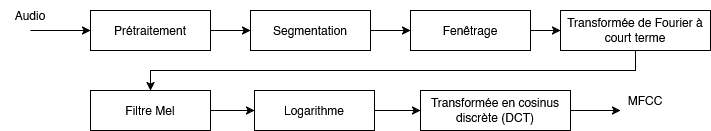
\includegraphics[width=0.95\textwidth]{images/mfcc.png}
	\caption{Algorithme d'extraction des MFCC}
\end{figure}
\end{center}
\paragraph{Pré-traitement}
Plus précisément, le pré-traitement consiste à prétraité le signal audio en appliquant un pré-emphase pour augmenter les hautes fréquences. Cela permet de réduire les problèmes liés à l'atténuation des hautes fréquences dans les systèmes de transmission. La formule de pré-emphase est la suivante :
\[
y[n] = x[n] - \alpha x[n-1]
\]
où $x(t)$ est le signal d'entrée, $y(t)$ est le signal de sortie et $\alpha$ est le coefficient de pré-emphase (généralement compris entre 0,95 et 0,97). 
\paragraph{La segmentation}
La segmentation consiste, elle, a divisé en trames le signal audio de taille fixe (généralement 20 à 40 ms) avec un certain chevauchement entre les trames adjacentes. Cette étape est nécessaire pour rendre compte de la nature non stationnaire des signaux audio.
\paragraph{Le fenêtrage}
Souvent nommé \textbf{Hamming} ou \textbf{Hanning} est appliquée à chaque trame pour minimiser les discontinuités aux bords de la trame. La fenêtre est définie comme suit :
\[
w[n] = \frac{1}{2}(1 - cos(\frac{2 \pi n}{N - 1}))
\]
où $w(n$) est la valeur de la fenêtre à l'échantillon $n$ et $N$ est la taille de la trame.
\paragraph{FFT}
La Transformée de Fourier à court terme (STFT) est appliquée à chaque trame pour obtenir le spectre de puissance. Cette étape permet de passer du domaine temporel au domaine fréquentiel. 
\paragraph{Les filtres Mel}
Ils sont calculés à l'aide d'un banc de filtres en triangle espacés selon l'échelle de fréquence Mel. L'échelle Mel est une échelle de fréquence perceptuelle qui tient compte de la manière dont l'oreille humaine perçoit les fréquences. La relation entre la fréquence Mel m et la fréquence linéaire f est la suivante :
\[
m = 2595 \times \text{log}10(1 + \frac{f}{700})
\]
Le \textbf{logarithme} de l'énergie de chaque filtre Mel est calculé. Cette étape permet de compresser les données en réduisant l'échelle dynamique.
\paragraph{DCT}
Pour finir, la Transformée en cosinus discrète (DCT) est appliquée au spectre log-Mel pour obtenir les coefficients MFCC.

Avant de passer à l'algorithme nous devons découper notre audio en frame de 256 échantillons. Mais pour ne pas perdre le maximum d'informations nous devons les superposer pour en quelques sorte garder l'effet "continu" de l'audio. On sait que notre enregistrement fait au total 8000 échantillons puisque nous voulons enregistrer 1 seconde (avec une fréquence de 8KHz). Nous avons vu sur les données que le professeur avait déjà enregistrer (\href{https://github.com/ElectroniqueECE/Projet_ING3/blob/main/training.txt}{\texttt{training.txt}} de ElectroniqueECE) qu'il y aura 48 lignes de 13 coefficients. Nous voulons garder et avoir la même logique pour pouvoir entraîner et obtenir des résultat cohérents par la suite. Désormais nous pouvons calculer combien d'échantillons nous devons superposer. Voici le schéma de la situation : 
\begin{figure} [H]
	\centering
	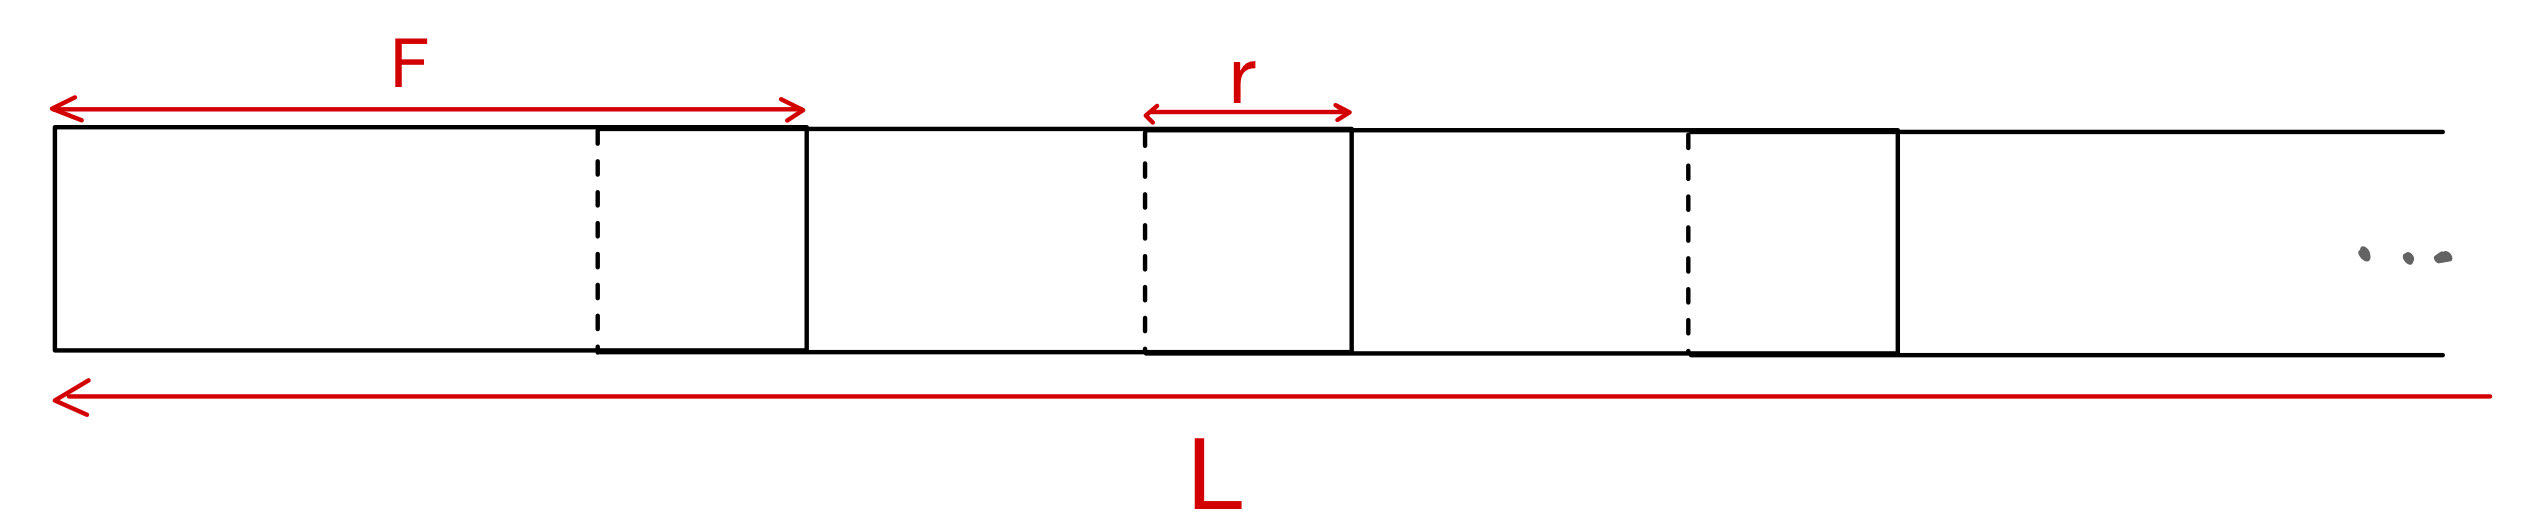
\includegraphics[width=0.7\textwidth]{images/recouvrement.jpg}
	\caption{Schéma montrant le recouvrement, avec $F$ le nombre d'échantillons dans une frame, $L$ le nombre total d'échantillons dans l'enregistrement, $r$ le recouvrement qu'on cherche.}
\end{figure}
D'après le schéma suivant nous pouvons déterminer plus facilement la superposition : 
\[
	L = FN - r(N-1)
\]
Alors on isole $r$ le "hop-length" et on obtient : 
\begin{equation}
	r = \frac{FN - L}{N-1}
\end{equation}\label{eq:recouvrement}
Ainsi, on sait que dans notre cas on a $F = 256$, $N = 48$ et $L = 8000$. Donc, on a :
\[
	r = \frac{256 \times 48 - 8000}{47} \approx 91.2
\] 
Ainsi le nombre d'échantillons entre une frame à une autre peut se trouver facilement suivant la formule suivante :
\[
	F - r \approx 256 - 91.2 \approx 164
\]
On connait maintenant le recouvrement, nous pourrons le mettre dans l'algorithme afin de garder seulement les frames qui nous intéresse. Nous appliquons alors l'algorithme MFCC qui va nous transformer chacune de nos 48 frames de 256 échantillons en 48 frames de 13 coefficients, ce qui nous réduit considérablement la taille de notre enregistrement. De plus, grâce à cette technique, nous pourrons en quelque sorte transformer notre audio en une image reconnaissable (voir figure \ref{fig:visu_mfcc}). Nous avons le choix alors d'appliquer la dernière étape DCT, pour notre cas, ça allait réduire considérablement le nombre d'entrée ($624 \rightarrow 288$ car matrice de $48 \times 6$). Nous avons fait les tests entre les deux et nous avons pas vu de réelle différence. Alors nous avons fait le choix de garder les coefficients MFCC au lieu de DCT pour qu'on arrive mieux à les visualiser.

\subsubsection{Enregistrement des données d'entraînement}

Désormais, nous voulons prendre toutes les données après l'algorithme MFCC pour pouvoir les traiter dans le réseau de neurones pour nous donner une prédiction. Pour simplifier la mémoire de la carte nous avons déjà décider d'entrainer notre réseau de neurones directement sur TensorFlow ce qui nous éviterai d'avoir un très petit modèle qui ne prend pas beaucoup d'espace sur la carte. De plus nous avons vu et manipulé les réseaux de neurones durant les TP et nous avons vu que pour améliorer la performance il y avait beaucoup d'optimisateur via le Github de la bibliothèque \href{https://github.com/GiorgosXou/NeuralNetworks}{\texttt{NeuralNetworks}} de Giorgos Xou \cite{neural}. Par exemple, passer pour la mémoire EEPROM, utiliser la mémoire PROGMEM au lieu de RAM etc... Ainsi notre choix se focaliserai principalement sur TensorFlow via Python, mais pour cela nous devons extraire toutes les données dans des fichiers textes pour pouvoir l'exporter directement dans notre programme Python. Nous allons les inscrire dans le Serial que nous allons récupérer grâce au logiciel PuTTY. Nous gardons les techniques vues dans la section \ref{traitement} pour enregistrer nos données puisque nous devons utiliser le microphone. Nous implémenterons un bouton poussoir pour indiquer que le locuteur est prêt à parler et ensuite nous utiliserons une LED qui restera allumé pendant toute la durée de l'enregistrement. Ce choix nous évitera d'avoir le bruit du bouton ou alors la différence de temps lorsque le locuteur appuie et parle. Nous gagnerons en précision notamment parce que le temps de réaction d'un humain est très similaire (environ 200 - 300ms) ce qui signifie que si l'enregistrement dure 1 seconde, le son du mot sera parfaitement au centre de l'enregistrement total. Voici l'algorigramme complet de notre code pour enregistrer les valeurs : 
\begin{figure}[H]
\centering
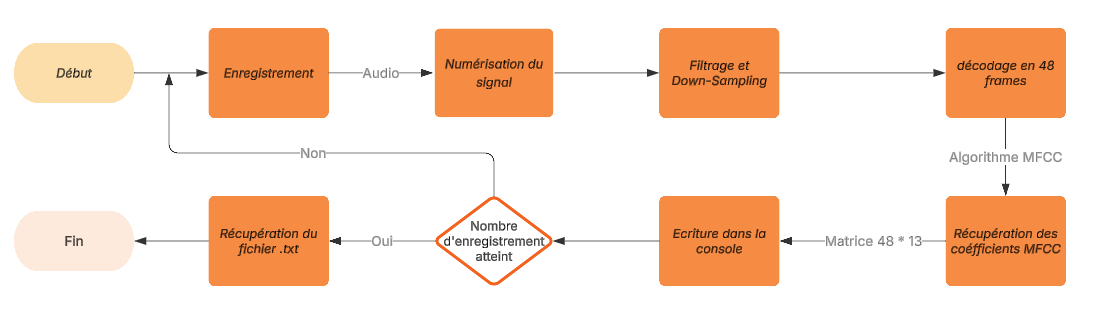
\includegraphics[scale=0.5]{images/algo_enregistrement.png}
\caption{Algorigramme pour enregistrer nos données} \label{fig:algo_enregistrement}
\end{figure}

\subsection{Réseau de neurones} \label{dev:reseau}

Dans cette partie nous allons voir comment on a mis en place notre réseau de neurones. Nous avons commencé directement à coder sur Python à l'aide de la librairie \href{https://www.tensorflow.org/}{\textbf{TensorFlow}} \cite{tensorflow}, parce que nous nous sommes dit que ça allait être plus pertinent et plus rapide d'entraîner sur une machine externe. Nous avons aussi eu l'ambition de mettre plus que deux couleurs et d'améliorer la précision au maximum pour être robuste et pouvoir prédire des couleurs avec n'importe quelles voix.

\subsubsection{Complexité des convolutions} \label{convolutions}
Nous avons d'abord penser à mettre plusieurs couches de convolutions pour que la machine puisse reconnaître des caractéristiques uniques dans les MFCC. Mais le problème avec cette méthode est qu'il y aura besoin de beaucoup de couches de convolutions ce qui entraînera un plus lourd traitement sur la carte. En effet, les formules qu'on utilise le \texttt{padding} ) 'same' ce qui ne réduit pas l'image. Par exemple si nous appliquons deux couches de convolutions avec deux max-pooling on aura la taille suivante : 

\begin{table}[H]
\begin{center}
\begin{tabular}{lc}
\toprule
\textbf{Couche} & \textbf{Dimension de la sortie} \\
\midrule
Convolution 2D & (48, 13, 64) \\
Max-pooling 2D & (24, 6, 64) \\
Convolution 2D & (24, 6, 32) \\
Max-pooling 2D & (12, 3, 32) \\
Flatten & (1152) \\
Sortie & (1) \\
\bottomrule
\end{tabular}
\end{center}
\caption{Application des différentes couches de convolutions}
\end{table} 
On peut voir que pour chaque couches de convolutions on applique 64 kernels (ou 32 pour la deuxième couches) ce qui signifie que nous devrons manipuler dans le code Arduino des tableaux de $48 \times 13 \times 64$ ce qui dépasse complètement la mémoire de la carte. Si nous mettons une couche de convolutions avec un filtre appliqué, lorsque nous le testons sur TensorFlow, nos résultats ne sont pas concluant et mettent beaucoup trop longtemps à converger, voir complètement diverger. Pour trouver la bonne combinaison nous avons besoin de faire du fine-tuning et faire des sacrifices pour avoir une bonne rapidité tout en ayant des résultats performant. C'est ainsi que nous avons fait le choix de ne pas utiliser de convolutions.

\subsubsection{Entraînement}
\paragraph{Normalisation}
Pour entraîner notre réseau de neurones, nous avons d'abord dû normaliser nos données. En effet les données varient entre 1.5 et à peu près 4.5. Pour cela nous allons simplement normaliser grâce à la formule suivante : 
\begin{equation}
	x_{\text{norm}} = \frac{x_{\text{brut}} - \mu}{\sigma}
\end{equation}
Avec $\sigma$ l'écart-type de toutes les valeurs du tableau, $\mu$ la moyenne, $x_{\text{norm}}$ les nouvelles valeurs après normalisation et $x_{\text{brut}}$ les anciennes valeurs non normalisées. Ainsi nous allons appliquer cette formule pour l'entraînement mais aussi pour la prédictions car nous devons respecter le même format de nos données. 

\paragraph{Shuffle}
En plus de la normalisation des données nous avons aussi mis une fonction \texttt{shuffle} pour mélanger l'ordre de nos données d'entraînement. En effet, si nous entraînons notre réseau de neurones avec un ordre bien précis notre réseau pourrait commencer à apprendre l'ordre des réponses. Même si nous savons que nous avons un petit dataset avec un réseau de neurones simple, si nous ajoutons cette fonctionnalité nous pourrons améliorer notre précision.

\paragraph{Les couches de convolution du réseau de neurones}
Après que les données ont été préparé et normaliser, nous pourrons les mettre dans le réseau de neurones mais nous devons d'abord réfléchir sur la structure du réseau de neurones. Pour cela nous avons pensé à plusieurs architecture incluant les convolutions, les couches denses et d'autres techniques comme par exemple les pooling. Au départ nous sommes partis sur double couches de convolution avec des couches profondes comme le présente le schéma ci-dessous: 
\begin{figure}[H]
\begin{center}
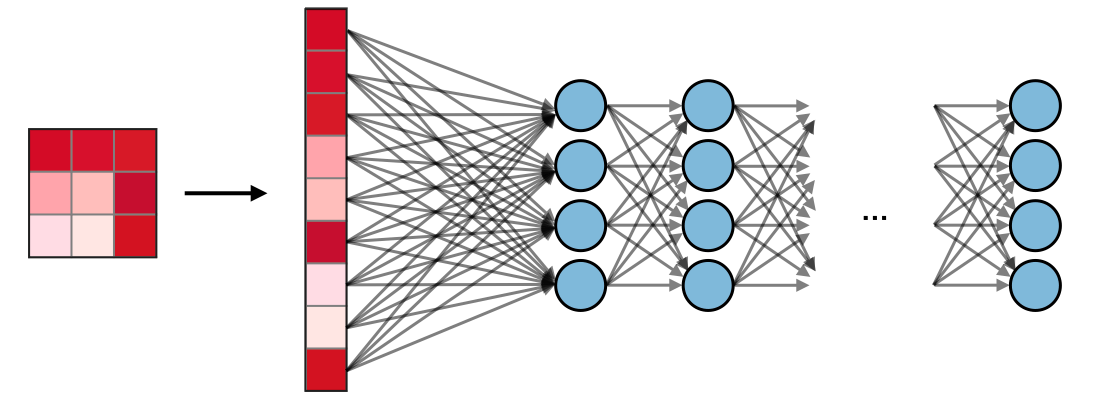
\includegraphics[scale=0.3]{images/cnn1.png}
\caption{Exemple d'un réseau de neurones convolutionnel profond}
\end{center}
\end{figure}
Mais comparé à notre application que nous devons faire et ainsi le problème vu dans la section \ref{convolutions}, nous avons pensé que notre réseau de neurones n'avait pas besoin d'être autant complexe sachant qu'on a une carte avec une mémoire limité et que nous avons pas beaucoup de données à entraîner (beaucoup moins de 5000). C'est ainsi que notre choix était sur un réseau de neurones simple.

\paragraph{Les couches de notre réseau de neurones}
Comme vu à la section \ref{mfcc}, nous avons fait le choix de garder seulement les coefficients des MFCC, on aura alors en entrée $48 \times 13 = 624$ entrées, et 4 sorties car nous aurons une led par couleurs (bleu, rouge et verte) et une led en plus pour indiquer l'erreur (on développe cette partie dans la section \ref{erreur}). Nous devons à présent choisir l'architecture de notre réseau de neurones en faisant des essais. C'est ainsi que nous allons le développer le choix du nombre de couches profondes et tous les choix concernant l'architecture de notre modèle dans la partie \ref{neuralnetworks}. Par ailleurs nous pouvons déjà construire l'algorigramme de notre code Python nous permettant d'entraîner notre réseau de neurones : 
\begin{figure}[H]
\begin{center}
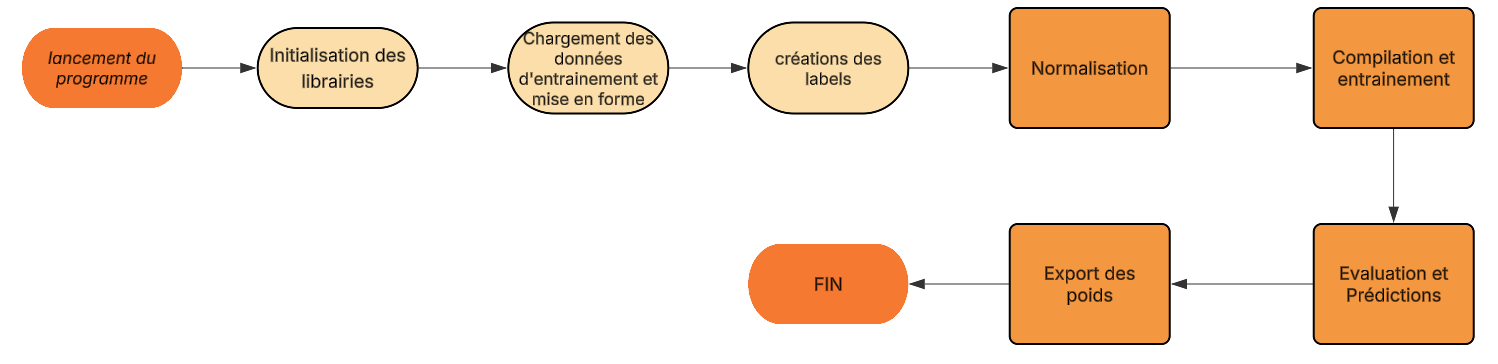
\includegraphics[scale=0.35]{images/algo_cnn.png}
\caption{Algorigramme de notre code pour entraîner notre réseau de neurones} \label{fig:algo_cnn}
\end{center}
\end{figure}

\paragraph{Liaison avec l'Arduino Due}
La liaison est très basique, nous affichons tout simplement les poids de notre réseau de neurones déjà entraîné sur la console de notre programme Python à l'aide de la fonction TensorFlow \texttt{model.get\_weights()}. Grâce à cette fonction nous pourrons récupérer les poids déjà entraîner de notre réseau de neurones sur TensorFlow puis les coller dans notre réseau de neurones sur la carte Arduino Due.

\subsection{Prédictions}
Cette partie est la dernière de notre projet, elle concerne la mise en application de notre réseau de neurones. Nous allons rassembler toutes les parties de ce projet pour l'implémenter dans un seul code Arduino pour faire les prédictions directement sur celle-ci. Pour cela nous allons reprendre bloc par bloc pour former un code final qui va permettre de faire la prédictions de plusieurs couleurs. Voici l'algorigramme simplifié de notre code de prédictions final : 
\begin{figure}[H]
\centering
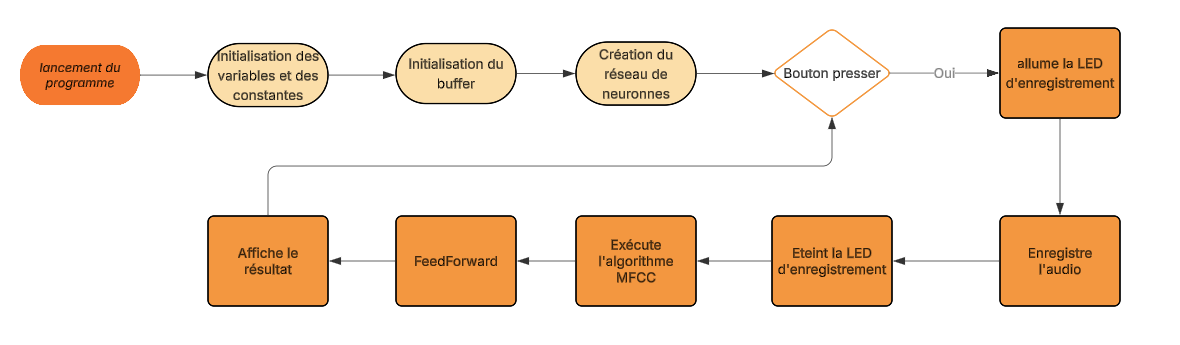
\includegraphics[scale=0.5]{images/algo_prediction.png} 
\caption{Algorigramme de notre code de prédictions}\label{fig:prediction}
\end{figure}

\subsection{Bonus}
Pour que notre projet soit 100\% en embarqué nous avons décidé de mettre tout notre système dans une boîte fermée avec seulement les leds et le boutons qui sont apparents puis le tout sera branché à une batterie externe qui délivra 5V à notre carte avec le code de la prédictions déjà implémentée sur celle-ci. Voici un croquis de notre construction finale : 
\begin{figure}[H]
\begin{center}
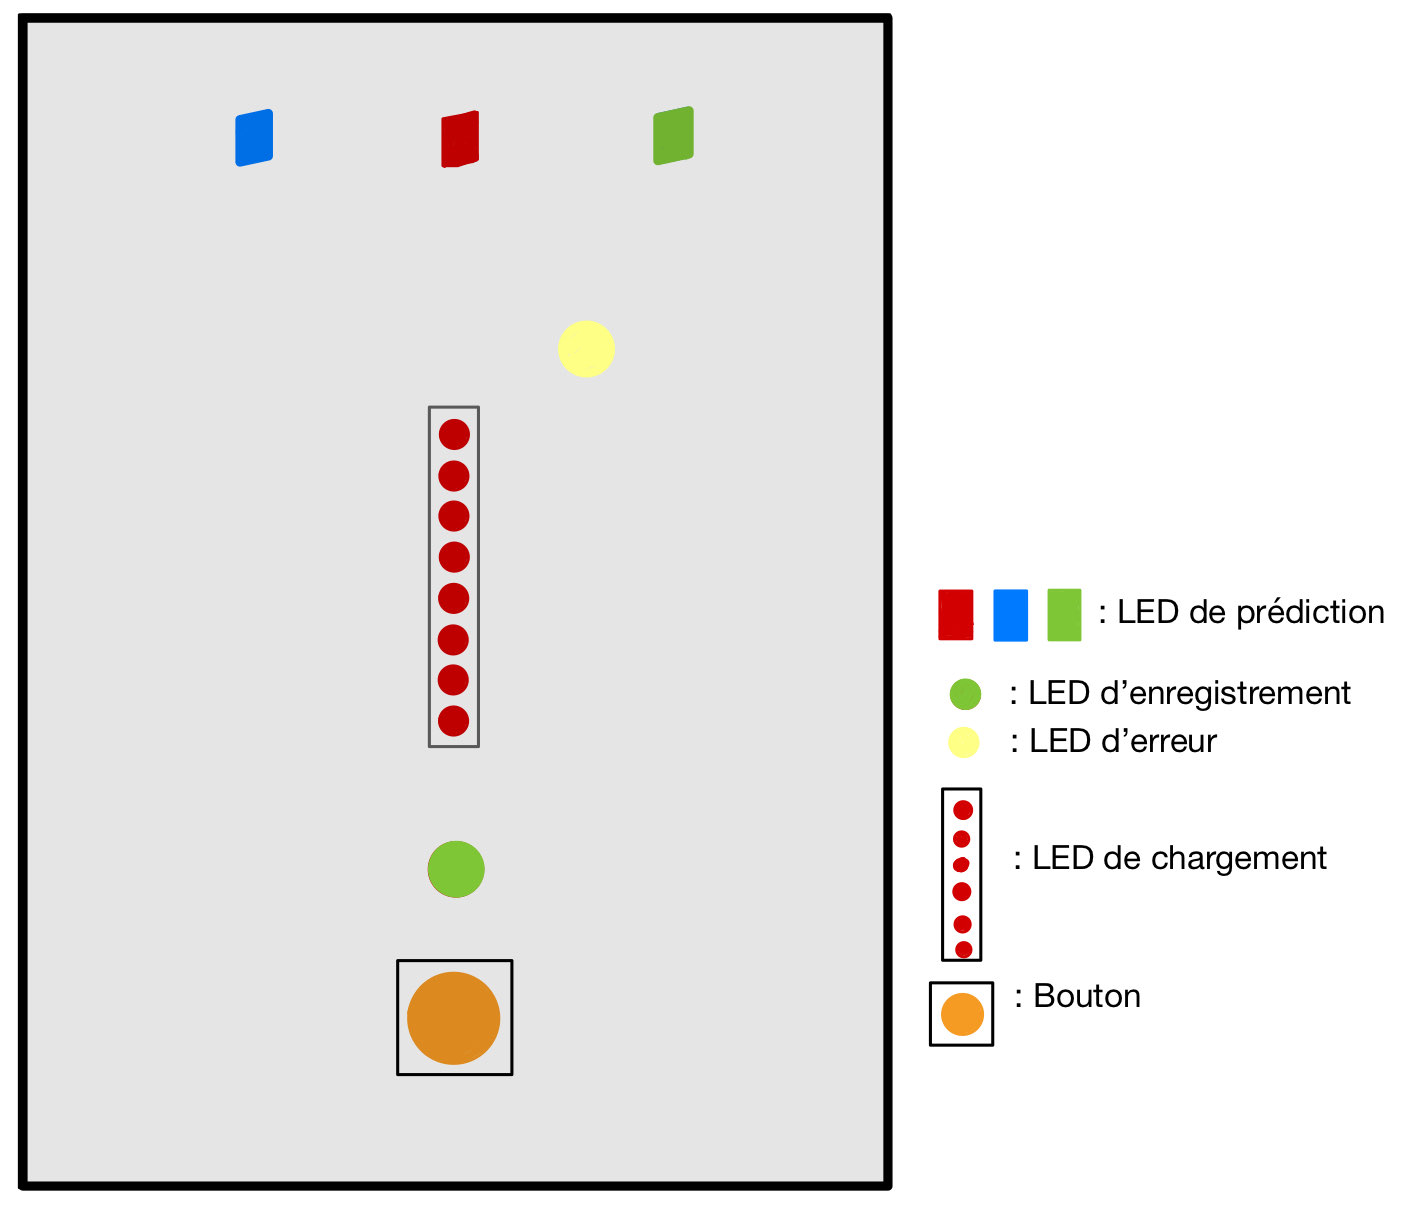
\includegraphics[scale=0.15]{images/boite.jpg}
\caption{Croquis de notre boîte final avec l'alimentation à l'intérieur. (Vue de dessus)}
\end{center}
\end{figure}

\subsubsection{Ajout d'une couleur}
Comme on l'a dit dans la section \ref{dev:reseau} nous voulions rajouté plus d'une couleurs et de pouvoir reconnaître le locuteur qui est en train de parler. Pour cela, nous devons plus de données enregistrer par chacun de nous et les stocker bien comme il faut. Pour reconnaître les couleurs, nous avons rajouté des sorties, ainsi, si nous voulons ajouter $n$ couleurs, il nous faudra rajouter $n$ sorties avec au moins $50n$ enregistrements en plus. 

\subsubsection{Reconnaissance du locuteur}\label{locuteur}
Concernant cette partie, le but ici sera de reconnaître le locuteur qui est en train de parler. Pour se faire nous avons rajouter un autre réseau de neurones parallèle à celui des couleurs et nous l'avons entrainé de la même manière sauf qu'au lieu de lui apprendre les couleurs nous lui avons appris à différencier entre les voix. Ainsi, en sortie du réseau de neurones nous aurons $n$ neurones pour $n$ locuteurs différent. Comme nous avons rajouté un neurones nous devrons logiquement entraîner la voix de chacun pour que la machine puisse apprendre la voix de chacun. 

\subsubsection{Optimisation} \label{erreur}
Nous avons aussi implémenter la fonctionnalité du mot qui n'existe pas dans le dataset de base. Pour ce faire nous avons décider d'enregistrer plus de mots à entrainer en accentuant sur les mots connus de la langue française. Et ensuite nous allons les connecter à un neurones qui sera dédié aux "erreurs". Par exemple sur 50 mots inconnus, nous allons enregistrer 10 mots différents finissant par le son -er comme par exemple les verbes du premiers groupe, puis les 10 prochains les verbes du deuxième groupe en finissant par -ir, puis les 10 prochains sur des adverbes qui finissent en -ement puis les 10 prochains par des mots ordinaire, aléatoire et pour finir les 10 derniers par du vide ou alors du bruits de fonds. C'est avec cette technique que nous sommes performant sur tous les mots. De plus nous pourrons être très robuste sur des bruits de fond ou des mots qui ne sont pas des couleurs.

\section{Tests et validation}
	
\subsection{Traitement du signal}

\subsubsection{Numérisation}
D'après le développement de la section \ref{numeriser}, et d'après la formule \ref{eq:rc}, nous savons que notre $RC = 1312$, ainsi, nous ajoutons cette ligne : 
\begin{lstlisting} [language = c, label=code:num]
TC_SetRC(TC0, 0, 1312);
\end{lstlisting}
En faisant bien attention de sélectionner la \texttt{Clock1}. A l'issue de cette partie nous devons théoriquement obtenir un signal d'acquisition à 32 kHz. Pour le montrer nous allons le montrer grâce à l'oscilloscope et nous obtenons ces courbes : 
\begin{figure}[H]
\begin{minipage}{0.48\textwidth}
\centering
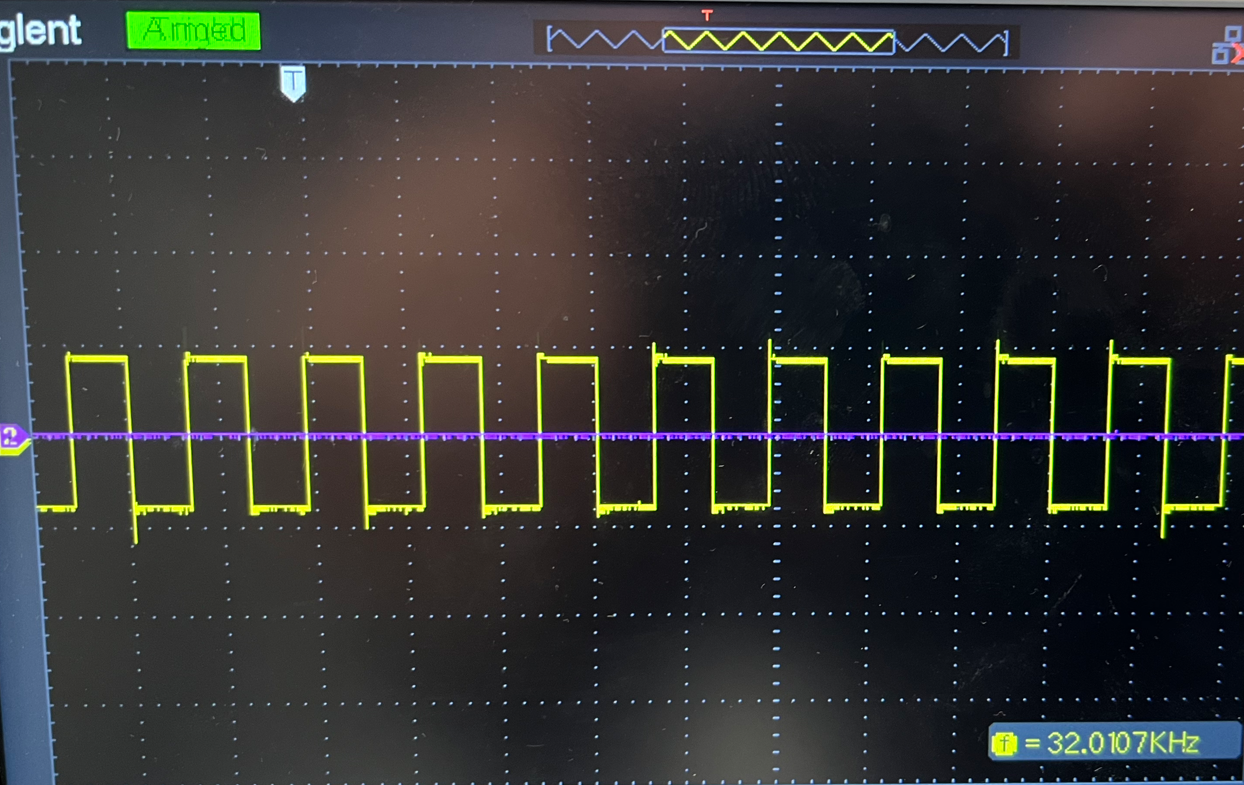
\includegraphics[scale=0.23]{images/numerisation1.png}
\end{minipage}
\hfill
\begin{minipage}{0.48\textwidth}
\centering
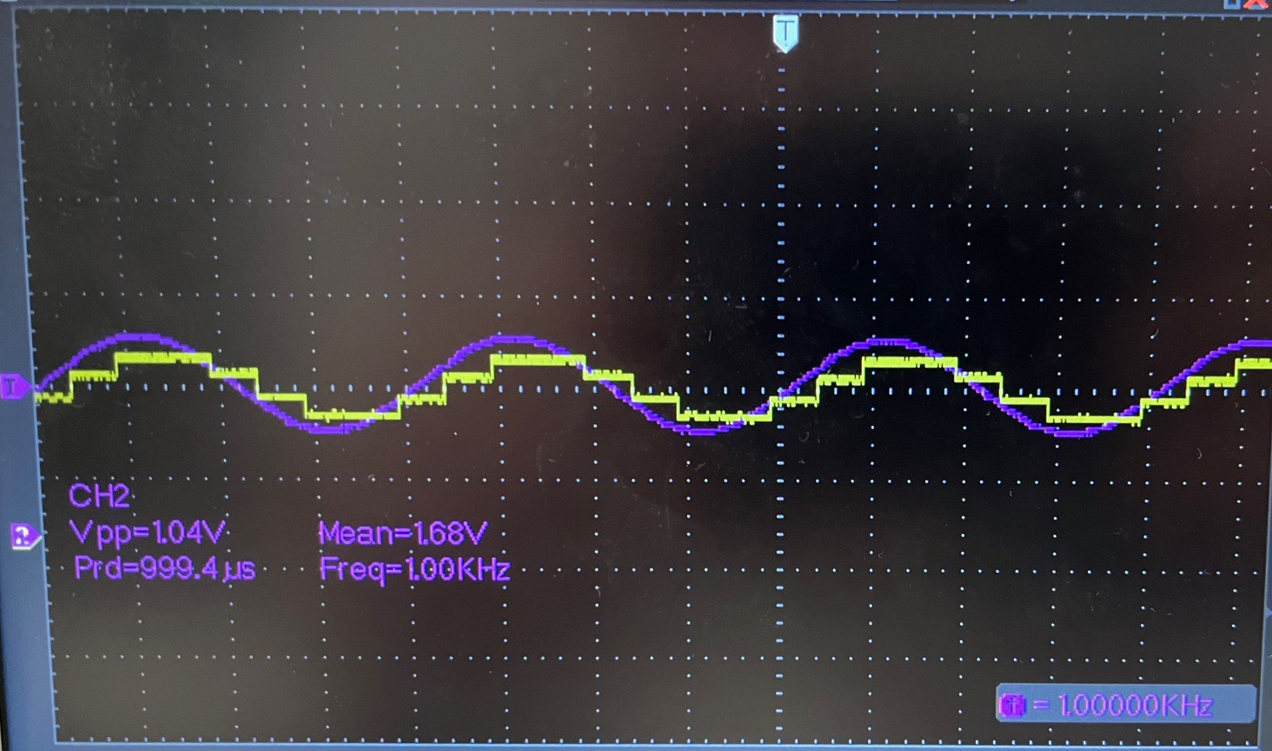
\includegraphics[scale=0.3]{images/escalier.png}
\end{minipage}
\caption{Validation du bon fonctionnement de notre signal d'acquisition 32 kHz} \label{fig:acquisition}
\end{figure}

D'après la figure \ref{fig:acquisition}, on peut voir le bon fonctionnement et l'obtention de la courbe à 32 KHz.

\subsubsection{Filtre RIF}
Concernant le filtre, d'après la section \ref{rif} nous voulons implémenter un filtre RIF. Pour cela, nous allons nous aider du site web \url{http://t-filter.engineerjs.com/} \cite{filtre2} pour trouver les coefficients nécessaires à l'implémentation du filtre. Sur ce site nous pouvons implémenter un filtre et récupérer directement les coefficients pour les transvaser directement dans notre code. Sachant que nous travaillons sur l'Arduino Due, nous avons une mémoire très limitée, c'est ainsi que nous avons réduit volontairement le nombre de coefficient qui étaient trop important à stocker dans notre tableau. Nous avons alors agrandi l'espace de la bande de transition du filtre. Ainsi nous nous retrouvons avec la courbe suivante pour valider l'efficacité de nos coefficients :

\begin{figure}[H]
\begin{center}
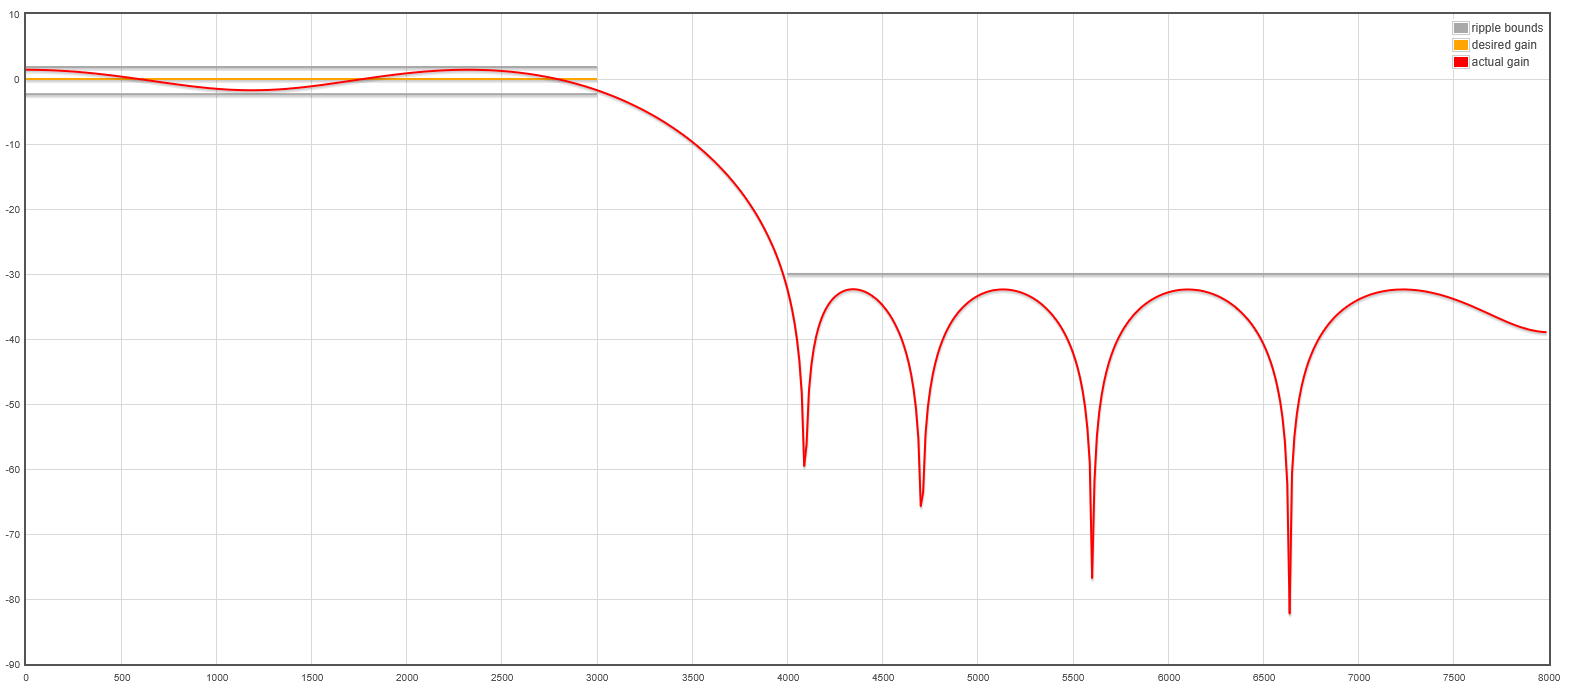
\includegraphics[scale=0.45]{images/rif3.png}
\caption{Courbe du filtre passe-bas RIF, qui atténue à partir de 4 kHz}\label{fig:freq_attenue}
\end{center}
\end{figure}
On peut voir sur la figure \ref{fig:freq_attenue}, qu'entre 3000 Hz et 4000 Hz, le signal est beaucoup atténué. Pour valider, nous allons tester grâce à l'oscilloscope et un GBF, pour cela, nous allons envoyer un signal de moins de 4 kHz et nous sommes censé obtenir en sortie notre signal non changé, et à l'inverse si nous mettons un signal de plus de 4 kHz nous devons obtenir notre signal atténué.

{\captionsetup{skip=0pt}
\begin{figure}[H]
\centering
\begin{minipage}[t]{0.45\textwidth}
\centering
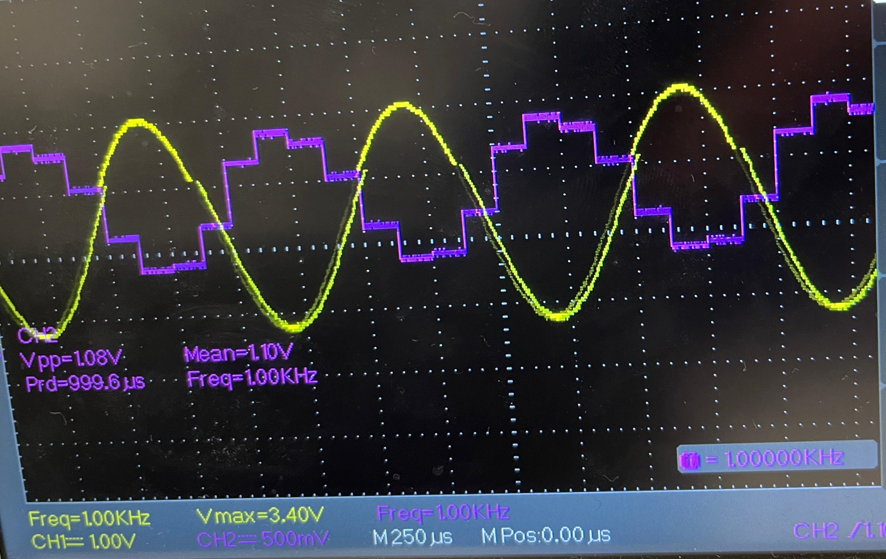
\includegraphics[height=4.2cm]{images/1khz.png}
\caption*{\textbf{(a)} Fréquence à 1 kHz}\label{fig:freq1}
\end{minipage}
\hspace{0.5cm}
\begin{minipage}[t]{0.45\textwidth}
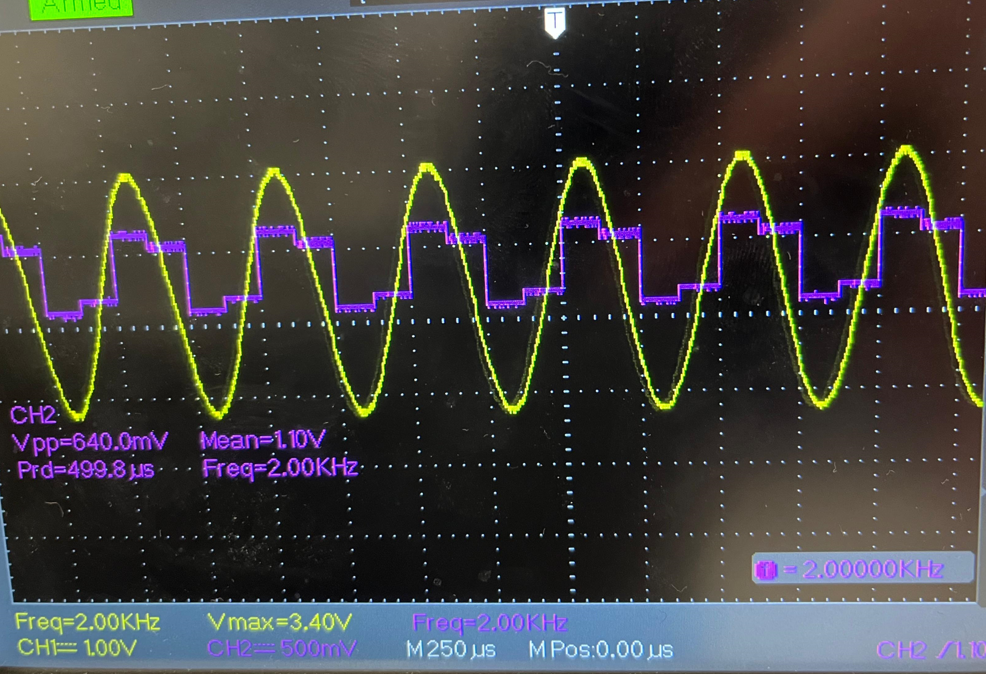
\includegraphics[height=4.2cm]{images/2khz.png}
\caption*{\textbf{(b)} Fréquence à 2 kHz} \label{fig:freq2}
\end{minipage}
\vspace{0.2cm}
\centering
\vspace{0.2cm}
\begin{minipage}[t]{0.45\textwidth}
\centering
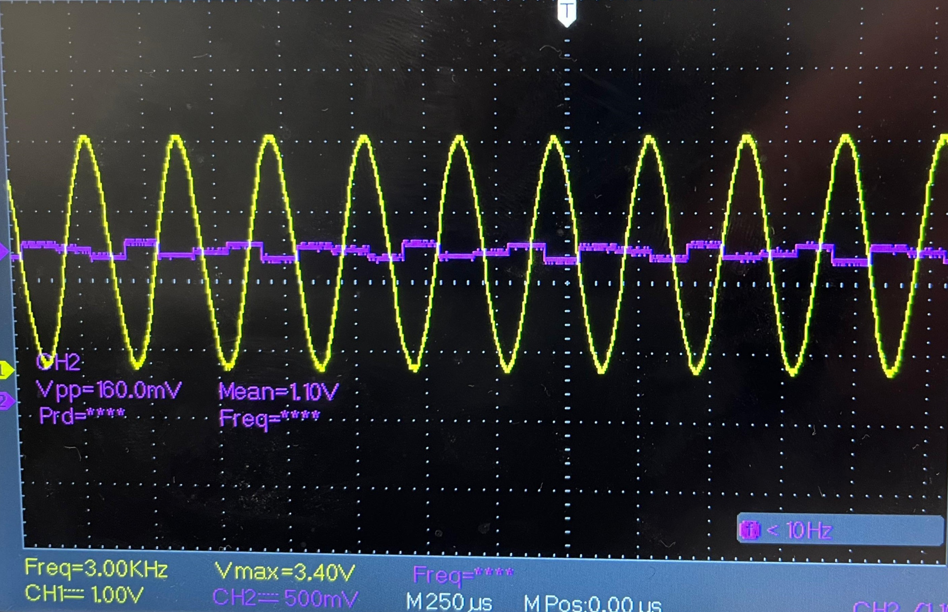
\includegraphics[height=4.2cm]{images/3khz.png}
\caption*{\textbf{(c)} Fréquence à 3 kHz}\label{fig:freq3}
\end{minipage}
\hspace{0.5cm}
\begin{minipage}[t]{0.45\textwidth}
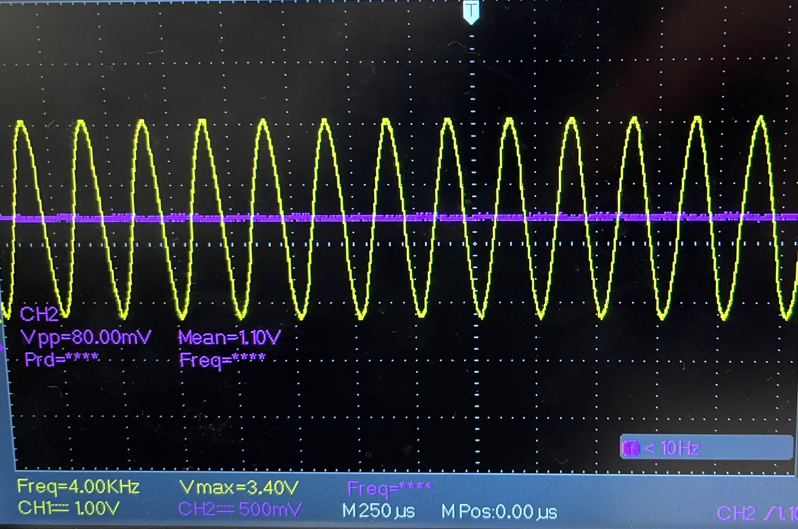
\includegraphics[height=4.2cm]{images/4khz.png}
\caption*{\textbf{(d)} Fréquence à 4 kHz} \label{fig:freq4}
\end{minipage}
\vspace{0.2cm}
\caption{Visualisation du filtre ainsi que le down-sampling} \label{fig:filtre}
\vspace{0.2cm}
\end{figure}
}

On voit bien sur la photo \textbf{(a)} de la figure \ref{fig:filtre}, le signal du GBF est à 1 kHz et que notre signal est échantillonné et avec qui on a appliqué un \textbf{down-sampling} (d'où le nombre de points inférieur à 32 kHz), on aperçois qu'elle suit bien la courbe jaune du GBF. Cela signifie qu'elle n'est pas filtré. Par ailleurs, plus on se rapproche de la fréquence 4 kHz, on aperçois que la courbe est totalement filtré (voir la photo \textbf{(d)} de la figure \ref{fig:filtre}. Avec la photo \textbf{(c)}, on voit que le filtrage se fait très tôt car on a un signal très atténué (mais pas 0 !) à 3 kHz, ce phénomène vient du fait qu'on a pris une distance de transition élevée (voir figure \ref{fig:freq_attenue}) pour éviter d'avoir trop de coefficient dans notre tableau Arduino. On peut conclure que notre filtre a bien été implémenté et notre down-sampling de $\dfrac{1}{4}$ de même. Grâce à ce filtre nous aurons plus de problème d'aliasing.

\subsubsection{Buffer circulaire}
Concernant le buffer-circulaire, comme expliqué dans la section \ref{buffer}, nous voulons stocker en continu des valeurs sans avoir à déplacer manuellement les éléments (ce qui économise du temps de traitement). Pour ce faire, pour valider que le buffer fonctionne correctement nous allons tout simplement afficher les valeurs de celui-ci dans la console. 

\begin{figure}[H]
\begin{center}
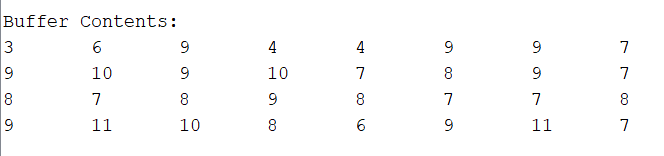
\includegraphics[scale=0.7]{images/buffer.png}
\caption{Affichage dans la console le bon fonctionnement du buffer circulaire}
\end{center}
\end{figure}

On peut alors valider le bon fonctionnement du buffer.

\subsection{Validation du bon fonctionnement du micro}
Pour cette partie, il était demandé de valider le bon fonctionnement du micro après les filtres, nous allons utiliser le logiciel \textbf{PuTTY} pour extraire toutes les données dans un fichier texte puis après nous allons, à l'aide d'un script Python, convertir les données \texttt{txt} en fichier \texttt{bin} pour que Audacity puisse lire les données en brute. Nous enregistrons notre voix en disant le mot électronique, et nous devons obtenir un audio où on l'entend correctement. 
\begin{figure}[H]
\begin{center}
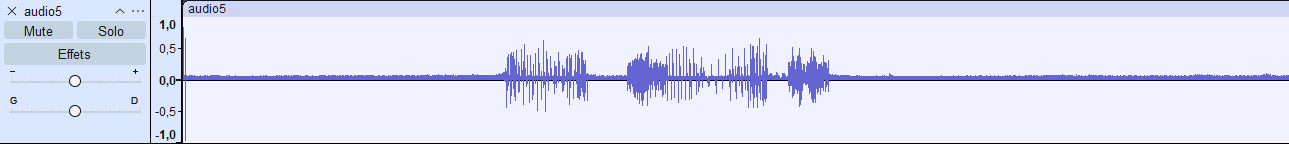
\includegraphics[width=15cm]{images/audacity3.png}
\caption{Exemple d'audio obtenu sur le logiciel Audacity}
\end{center}
\end{figure}
Pour conclure, on arrive bien à reconnaître notre voix en disant électronique même si celle-ci semble un petit peu modifié causés par les filtres et le down-sampling ajouté à notre signal audio. On peut conclure du bon fonctionnement des partie précédentes.

\subsection{Visualisation des caractéristiques sonores}

\paragraph{Découpage}
Comme on l'a dit dans la section \ref{mfcc}, on souhaite avoir à la fin de cette partie un tableau avec dimension $48 \times 13$ pour pouvoir ensuite le mettre dans notre réseau de neurones. Pour cela, nous découpons d'abord notre enregistrement en frame de 256 échantillons chacun. Puis nous savons le nombre de frame que nous désirons et ainsi grâce à l'équation \ref{eq:recouvrement} nous savons que nous voulons recouvrir nos frames avec 164 échantillons. Pour commencer, nous devons avoir un enregistrement d'une seconde, pour cela nous décidons de prendre seulement 8000 échantillons (parce que notre fréquence est à 8 kHz après le down-sampling). Nous validons cette opération grâce au logiciel \textbf{PuTTY} puis nous visualisons les données sur un logiciel d'éditeur de texte comme par exemple \textbf{Notepad++} et nous confirmons le nombres de lignes totales qui est de 8000. Après cette étapes, nous devons les découper en $N$ frames par 256 échantillons (48 dans notre cas), nous stockons les valeurs dans un tableau à 2 dimensions en faisant attention à respecter le bon nombre d'échantillons que nous recouvrons et nous vérifions maintenant que nous avons un double tableau avec 48 lignes et 256 échantillons par lignes. Nous vérifions les 91 échantillons qui se recouvrent et se partagent entre les frames. Nous effectuons le même teste que précédemment avec \textbf{PuTTY} et \textbf{Notepad++} et nous validons le bon fonctionnement du découpage. 

\paragraph{Algorithme MFCC}
Désormais, nous voulons appliquer l'algorithme des MFCC pour passer d'un tableau de dimension $48 \times 256$ en un tableau de $48 \times 13$. Pour cela, à chaque fois que nous allons calculer la frame actuelle nous allons exécuter cette commande dans notre boucle : 
\begin{lstlisting} [language = c, label=code_mfcc]
mymfcc.compute(frames[f], mfcc);
\end{lstlisting}
Avec \texttt{frames[f]} la frame actuelle et \texttt{mfcc} le tableau de sortie. Pour valider ce passage, nous allons afficher dans la console toutes les frames avec leur coefficients, on valide la bonne dimension de celle-ci. Maintenant, pour valider le bon fonctionnement de l'algorithme MFCC, nous allons visualiser les MFCC à l'aide du script Python qui a été donné lors des TP. On enregistre 2 fois les mots bleus, rouges et verts pour les comparer entre eux. Voici les enregistrement que nous obtenons: 

{\captionsetup{skip=0pt}
\begin{figure}[H]
\centering
\begin{minipage}{0.48\textwidth}
\centering
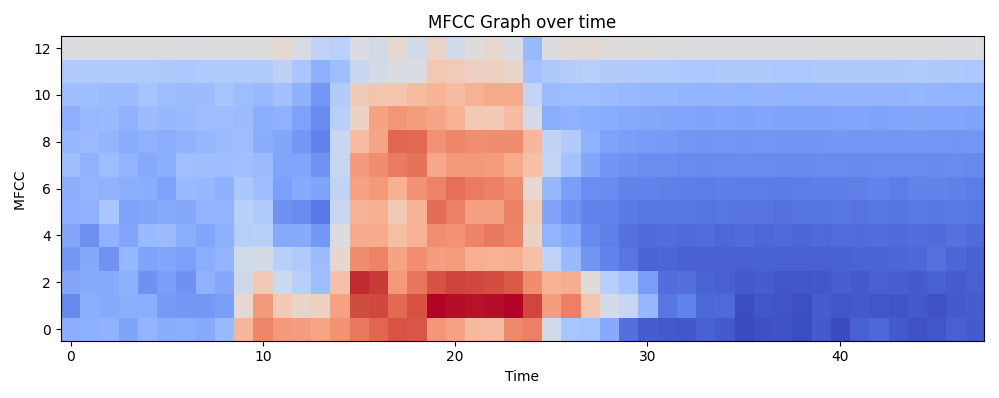
\includegraphics[scale=0.37]{images/bleu1.png}
\caption*{Bleu n°1}
\end{minipage}
\hfill
\begin{minipage}{0.48\textwidth}
\centering
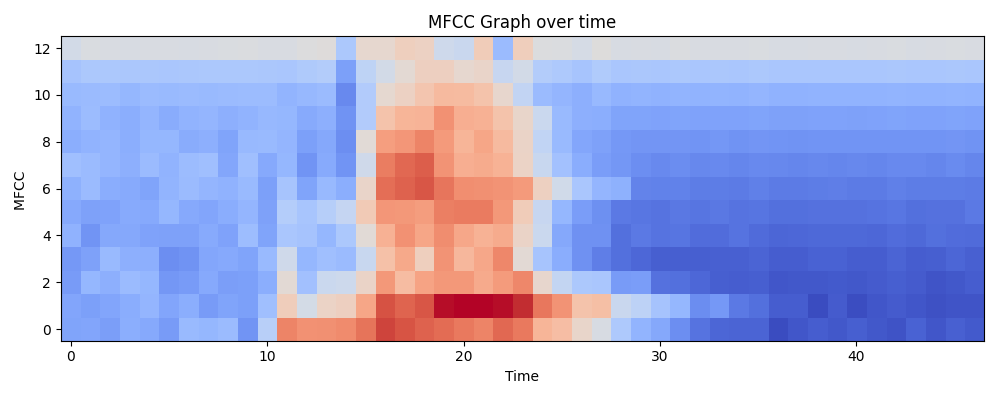
\includegraphics[scale=0.37]{images/bleu2.png}
\caption*{Bleu n°2}
\end{minipage}
\vspace{0.3cm}
\vfill
\begin{minipage}{0.48\textwidth}
\centering
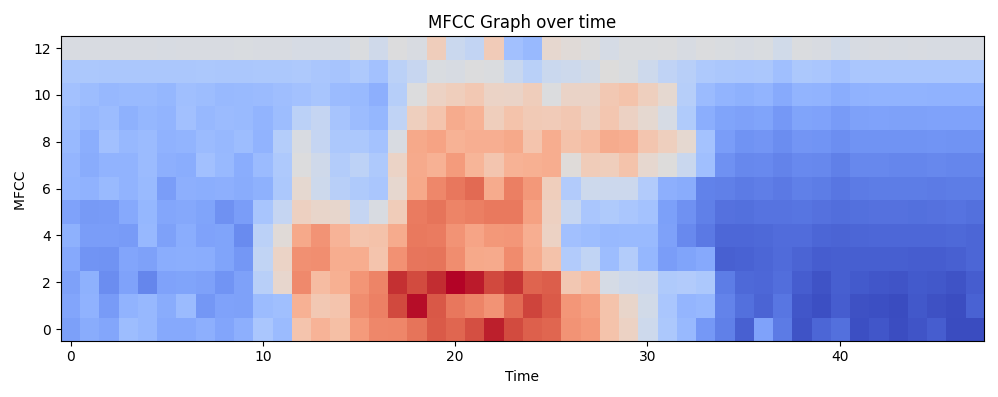
\includegraphics[scale=0.37]{images/rouge1.png}
\caption*{Rouge n°1}
\end{minipage}
\hfill
\begin{minipage}{0.48\textwidth}
\centering
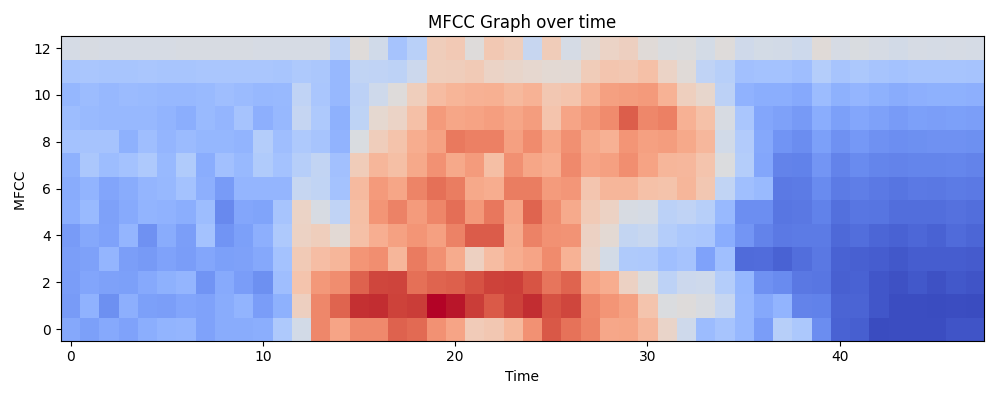
\includegraphics[scale=0.37]{images/rouge2.png}
\caption*{Rouge n°2}
\end{minipage}
\vspace{0.3cm}
\vfill
\begin{minipage}{0.48\textwidth}
\centering
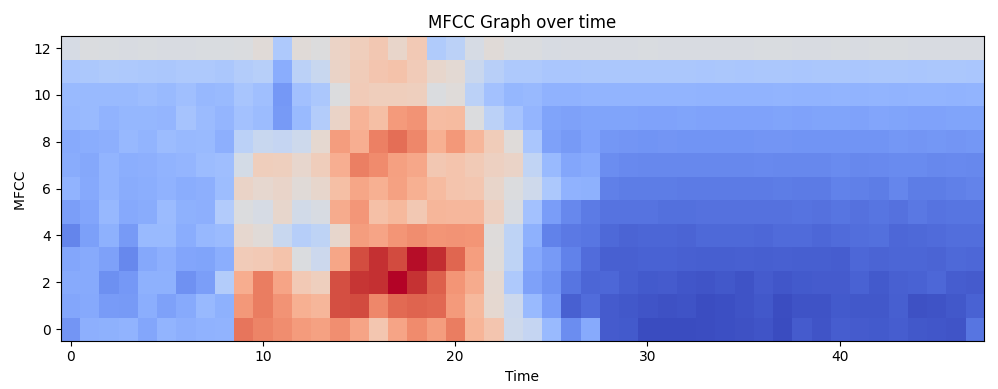
\includegraphics[scale=0.3]{images/vert1.png}
\caption*{Vert n°1}
\end{minipage}
\hfill
\begin{minipage}{0.48\textwidth}
\centering
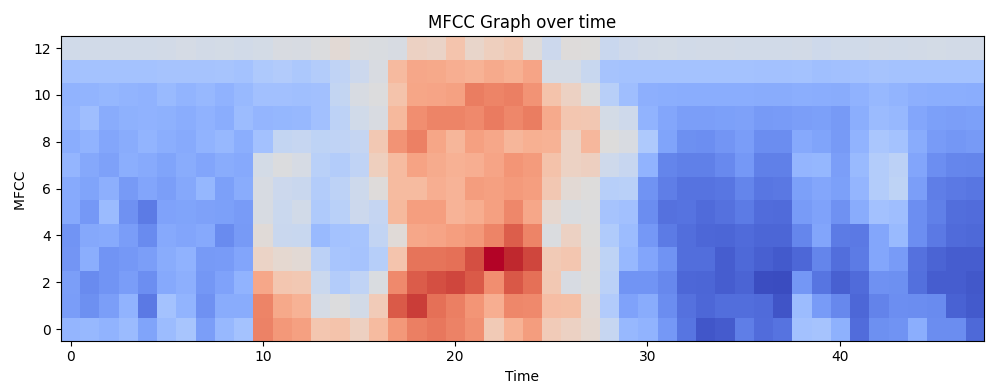
\includegraphics[scale=0.3]{images/vert2.png}
\caption*{Vert n°2}
\end{minipage}
\vspace{0.3cm}
\caption{Visualisation des MFCC enregistrés} \label{fig:visu_mfcc}
\end{figure}
}
On peut constater que les motifs sont bien issus d'enregistrements différents mais on arrive quand même à extraire certaines particularités entre les enregistrements bleus, rouges et verts, notamment par la forme de celle-ci. Même si nous les avons pas utilisé lors de notre réseau de neurones nous avons aussi visualisé la DCT sur un de nos enregistrement pour valider le bon fonctionnement de notre module et nous avons eu cette visualisation : 
\begin{figure}[H]
\centering
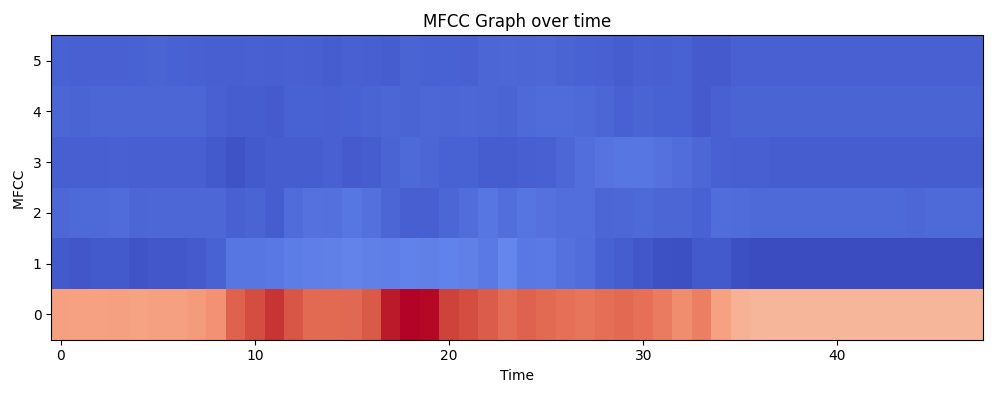
\includegraphics[scale=0.4]{images/dct.png}
\caption{Visualisation des coefficients après DCT. Ici il y a 6 coefficients.}
\end{figure}
Ainsi notre algorithme est bien prêt pour enregistrer nos données d'entraînement pour notre réseau de neurones.

\subsection{Réseau de neurones} \label{neuralnetworks}
\subsubsection{Réseau simple}\label{test:simple}
Maintenant que nous avons les MFCC prêt, nous avons enregistré d'abord 165 enregistrements (50 bleus, 50 rouges, 50 verts, et 5 de chaque pour les données de testes). Nous avons d'abord regardé comment réagirai nos prédictions si nous mettons un réseau de neurones très basique, c'est à dire, les couches d'entrées et les couches de sortie comme sur ce schéma : 
\begin{figure}[H]
\centering
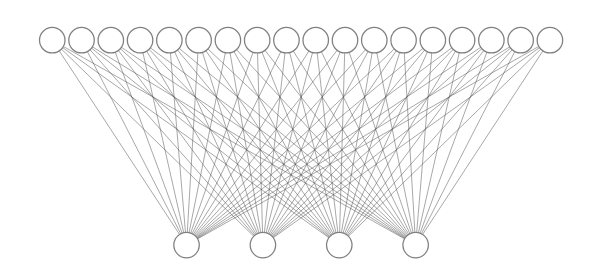
\includegraphics[scale=0.6]{images/cnn6.png}
\caption{Réseau de neurones basiques (624 entrées et 4 sorties) tourné horizontalement}\label{fig:simple}
\end{figure}
Et nous entraînons ce modèle sur 64 epochs et nous faisons nos prédictions sur nos données de tests et nous obtenons les précisions suivantes : 
\begin{table}[H]
\centering
\begin{tabular}{clccc}
\toprule
& \textbf{Mot testé} & \textbf{Bleu} & \textbf{Rouge} & \textbf{Vert} \\
\midrule
1 & Bleu & \texttt{0.9808915} & \texttt{0.0099078} & \texttt{0.0092007} \\
2 & Rouge & \texttt{0.0282434} & \texttt{0.9690930} & \texttt{0.0026637} \\
3 & Vert & \texttt{0.0012404} & \texttt{0.0000397} & \texttt{0.9987199} \\
\vdots & \vdots & \vdots & \vdots & \vdots \\
13 & Bleu & \texttt{0.8619314} & \texttt{0.0719171} & \texttt{0.0661516} \\
14 & Rouge & \texttt{0.0321044} & \texttt{0.9488044} & \texttt{0.0190913} \\
15 & Vert & \texttt{0.0157210} & \texttt{0.0104149} & \texttt{0.9738640} \\
\bottomrule
\end{tabular}
\caption{Prédictions pour un réseau de neurones simple}
\end{table}
Les prédictions sont correctes, pour évaluer l'erreur de notre réseau nous avons pensé que ça allait être plus optimale de regarder la précision sur nos données de tests (\texttt{accuracy} sur TensorFlow) et non la MSE car elle est linéaire. Durant l'entraînement, nous avons fait de la classification, du coup notre fonction de perte est la \texttt{categorical\_crossentropy} \cite{tensorflow}, qui fonctionne très bien pour des classification comme dans notre cas. Or dans ce cas nous avons seulement 5 données de tests par couleurs ce qui n'est pas assez pour avoir une précisions significative (notre précision est de 100\%, avec une perte en fin d'entraînement à 0.01). 

\subsubsection{Réseau complexe}
Pour pallier au problème de la partie \ref{test:simple}, nous avons enregistrer plus de valeurs pour nos entraînements pour espérer être plus précis. Nous avons aussi décider d'enregistrer les valeurs pour la LED d'erreur développé à la section \ref{erreur}. Nous avons réparti ainsi les enregistrement suivant ce tableau : 
\begin{table}[H]
\centering
\resizebox{\textwidth}{!}{ % Redimensionne le tableau à la largeur de la page
\begin{tabular}{lc *{13}{c}} 
  \toprule
  \multirow{2}{*}{} 
  & \multicolumn{3}{c}{\textbf{Axel}} 
  & \multicolumn{3}{c}{\textbf{Ethan}} 
  & \multicolumn{3}{c}{\textbf{Valentin}} 
  & \multicolumn{3}{c}{\textbf{Hugo}}
  & \multirow{2}{*}{\textbf{Erreur}}
  & \multirow{2}{*}{\textbf{Total}} \\
  \cmidrule(lr){2-4} \cmidrule(lr){5-7} \cmidrule(lr){8-10} \cmidrule(lr){11-13}
  & Bleu & Rouge & Vert 
  & Bleu & Rouge & Vert 
  & Bleu & Rouge & Vert 
  & Bleu & Rouge & Vert \\
  \midrule
  \textbf{Training} & 50 & 50 & 50 & 50 & 50 & 50 & 50 & 50 & 50 & 50 & 50 & 50 & 150 & \textbf{750} \\
  \textbf{Test}     & 5 & 5 & 5 & 5 & 5 & 5 & 5 & 5 & 5 & 5 & 5 & 5 & 15 & \textbf{75}\\
  \bottomrule
\end{tabular}
}
\caption{Répartition de nos enregistrements}
\end{table}

Avec ceci, nous prenons le même réseau de neurones que la figure \ref{fig:simple} et nous l'entraînons avec 50 epochs. Nous voyons que nous avons nos premières erreurs. En effet, 50 epochs n'étant pas assez pour 750 données en tout, alors nous décidons d'en mettre plus. Mais sur Python, nous obtenons de très bon résultat, par ailleurs, quand nous les essayons sur nos cartes, pour tester avec de nouvelles valeurs on voit que notre modèle n'est pas performant. Etant conscient du grand nombre d'epochs, nous avons décidé de complexifier notre réseau de neurones pour qu'il apprenne plus rapidement et avec plus de précisions. Ainsi nous avons ajouté deux couches de neurones profondes pour être avec \{624, 32, 12, 4\}.
\begin{figure}[H]
\centering
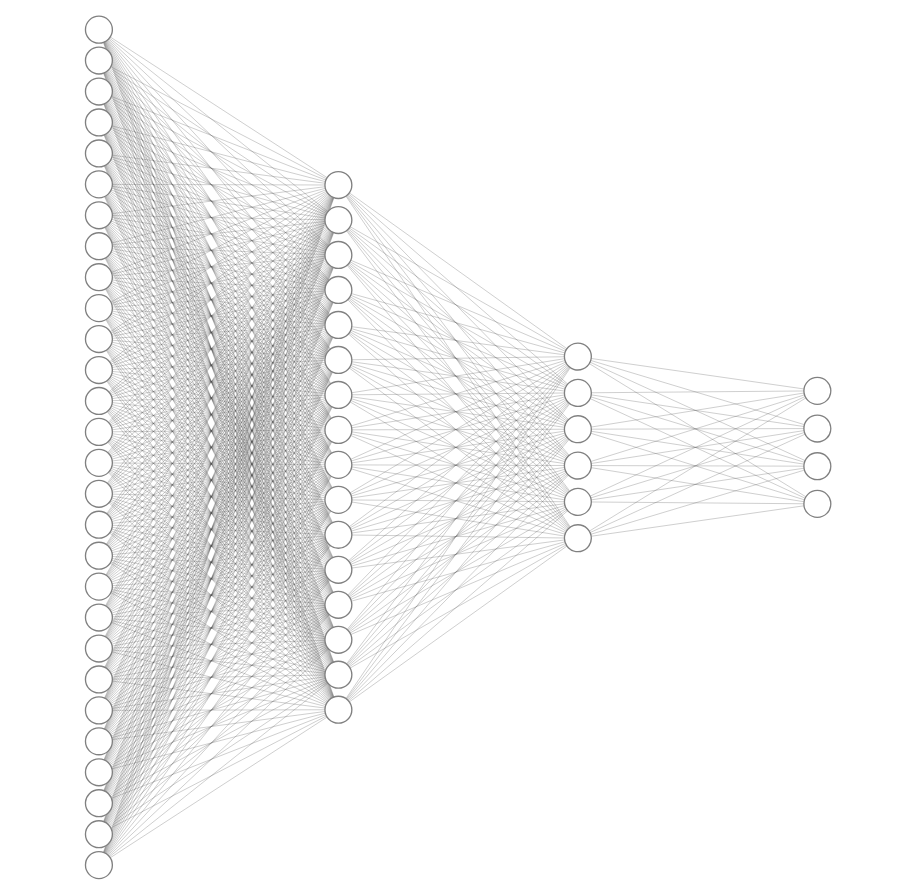
\includegraphics[scale=0.4]{images/cnn7.png}
\caption{Réseau de neurones plus complexe avec comme architecture \{624, 32, 12, 4\} (nous avons volontairement mis moins de neurones sur le schéma pour que ça soit compréhensible)}
\end{figure}
Or ici, lorsque nous faisons nos prédictions nous obtenons des résultats très convaincant pour la suite : 
\begin{table}[H]
\centering
\begin{tabular}{clcccc}
\toprule
& \textbf{Mot testé} & \textbf{Bleu} & \textbf{Rouge} & \textbf{Vert} & \textbf{Erreur} \\
\midrule
1 & Bleu & \texttt{0.9994659} & \texttt{0.0000060} & \texttt{0.0005232} & \texttt{0.0000049} \\
2 & Rouge & \texttt{0.0000307} & \texttt{0.9990181} & \texttt{0.0009508} & \texttt{0.0000005} \\
3 & Vert & \texttt{0.0000019} & \texttt{0.0001382} & \texttt{0.9998598} & \texttt{0.0000000} \\
4 & Erreur & \texttt{0.0000342} & \texttt{0.0024410} & \texttt{0.0000426} & \texttt{0.9974822} \\
\vdots & \vdots & \vdots & \vdots & \vdots & \vdots \\
72 & Bleu & \texttt{0.9995578} & \texttt{0.0004174} & \texttt{0.0000135} & \texttt{0.0000113} \\
73 & Rouge & \texttt{0.0011244} & \texttt{0.9988153} & \texttt{0.0000603} & \texttt{0.0000000} \\
74 & Vert & \texttt{0.0001200} & \texttt{0.0002301} & \texttt{0.9996244} & \texttt{0.0000255} \\
75 & Erreur & \texttt{0.0000175} & \texttt{0.0023316} & \texttt{0.0000843} & \texttt{0.9975666} \\
\bottomrule
\end{tabular}
\caption{Prédictions pour un réseau de neurones complexe}
\end{table}
Notre précision ici est de \textbf{98.46\%} avec une perte en fin d'entraînement de $<0.001$. Or ici, d'être trop précis nous questionne sur la possibilité d'être en sur-apprentissage et donc de ne pas être performant sur de nouvelles données. Pour être sûr nous avons décidé de tracer les courbes d'apprentissage pour suivre la tendance du \texttt{train\_loss}.
\begin{figure}[H]
\centering
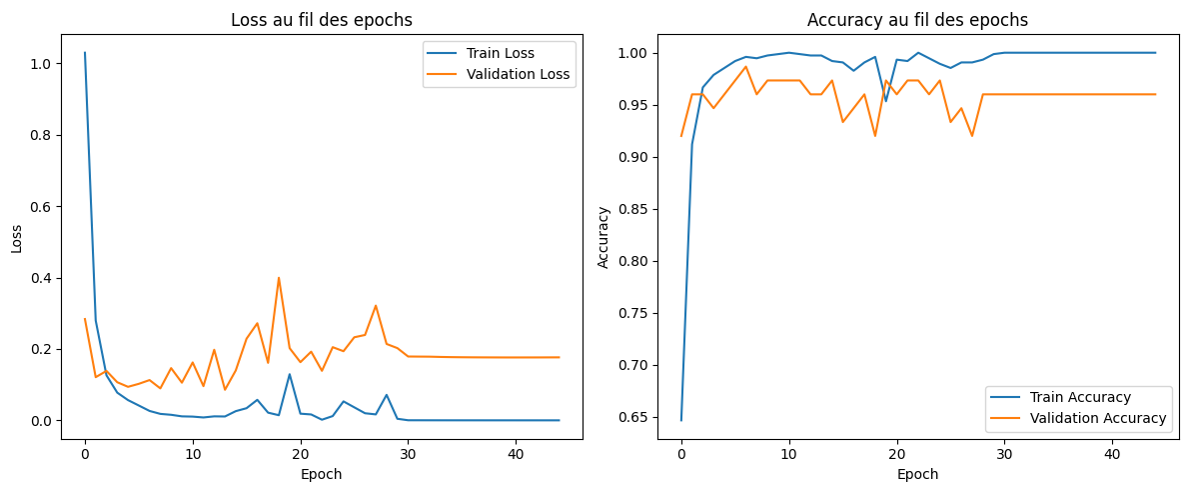
\includegraphics[scale=0.5]{images/overfitting1.png}
\caption{Courbes d'apprentissage nous montrant un sur-apprentissage}
\end{figure}
Pour pallier ce problème nous avons décider de d'abord ajouter le fonction TensorFlow \texttt{Dropout} \cite{tensorflow} qui permet de réduire le nombre de neurones volontairement en leur ajoutant du "bruit" pour que le réseau apprenne les vrais motifs et pas le motif précisément. De plus nous avons décidé de réduire la complexité tout en gardant une couche profonde tel le schéma suivant : 
\begin{figure}[H]
\centering
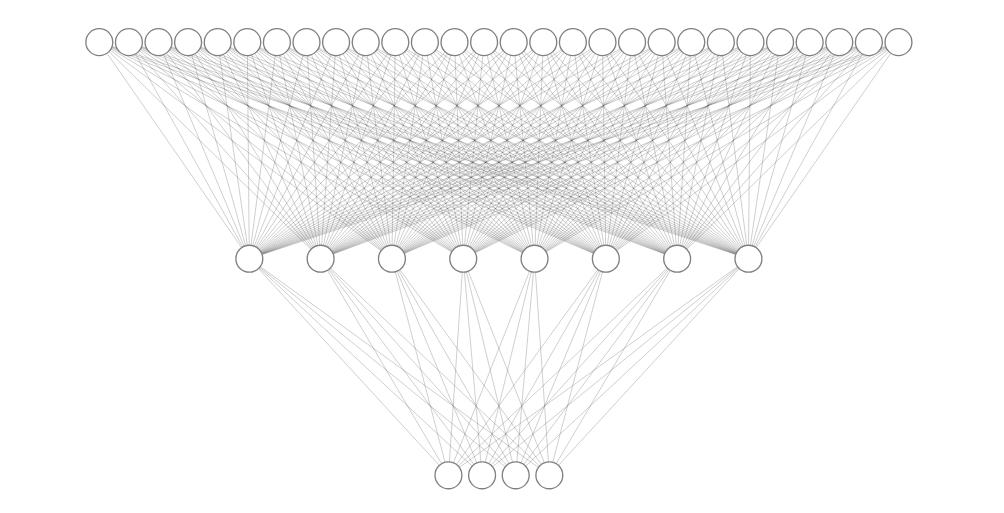
\includegraphics[scale=0.6]{images/cnn9.png}
\caption{Architecture du réseau de neurones avec seulement une couche profonde (réduite pour meilleur compréhension)}\label{fig:complex2}
\end{figure}
Nous retraçons les courbes d'apprentissage et nous voyons que les résultats sont bien meilleurs:
\begin{figure}[H]
\centering
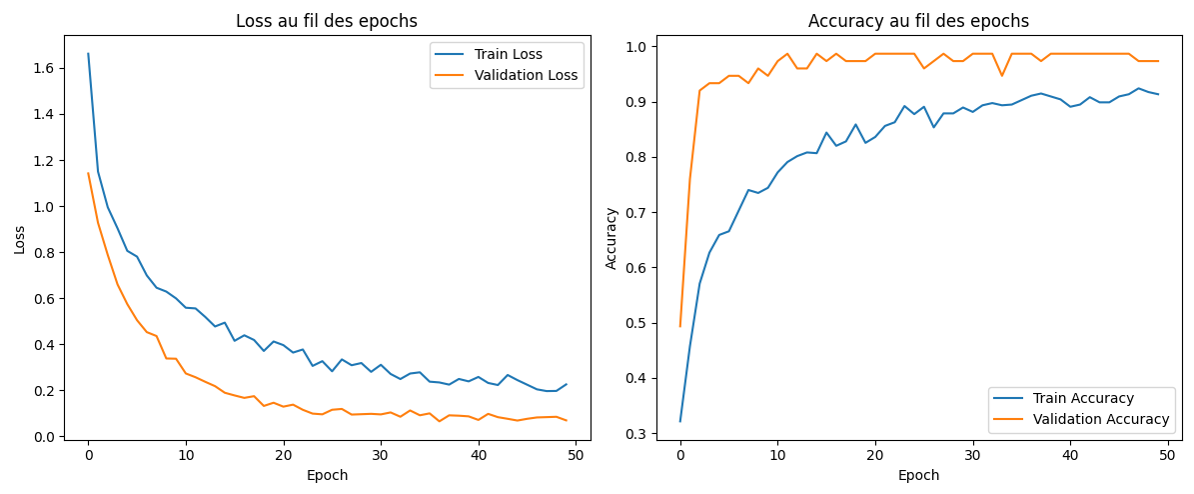
\includegraphics[scale=0.5]{images/loss_2.png}
\caption{Nouvelle courbe d'apprentissage associé à l'architecture de la figure \ref{fig:complex2}}
\end{figure}
Ainsi nous gardons ce réseau de neurones pour faire la prédictions sur la carte Arduino. Pour cela, on a juste à copier les poids ainsi que les biais sur la carte Arduino et utiliser seulement la fonction \texttt{FeedForward} de la bibliothèque \href{https://github.com/GiorgosXou/NeuralNetworks}{\texttt{NeuralNetworks}} de Giorgos Xou \cite{neural}. (voir l'algorigramme \ref{fig:prediction}). Nous obtenons ainsi une très bonne précision.

\subsubsection{Prédictions}
Après avoir notre réseau de neurones prêt et ensuite implémenter les poids sur la carte, nous avons fait 10 essais et les 10 essais ont été concluant et ainsi pu prédire chaque couleurs ainsi que la led d'erreur si nous disons rien dans le micro ou faisant du bruit de fond.
	
\section{Bilan}	
\subsection{État d’avancement}
Pour conclure, chaque partie de notre projet fonctionne parfaitement. Ce projet nous a passionné, ainsi nous sommes allé plus loin que ceux qui était demandé (ajout de couleur, ajout d'une led d'erreur, optimisation dans le traitement du signal en utilisant PROGMEM, optimisation de la performance en améliorant la précision de notre réseau de neurones). 
			
\subsection{Axe d'évolution et limite de notre solution}
Par ailleurs, nous avons constaté des petits points d'améliorations dans notre projet.
\paragraph{Plus d'enregistrements} 
Premièrement on pensait ajouter plus de données d'entraînement et aussi enregistrer des données de tests indépendamment des données d'entraînement, en effet, lorsque nous enregistrons les données d'entraînement nous enregistrons les données de test juste après, ce qui fait qu'on était dans la même pièce avec les mêmes conditions. Ainsi, si nous sommes dans une pièce avec beaucoup de résonance ce n'est pas la même que si nous sommes dans une pièce sans petit bruit de fond. Ainsi pour pallier ce problème, nous avons deux solutions, soit améliorer et faire une étude encore plus poussé du traitement du signal et / ou entraîner avec d'autres personnes. Le nombre de personnes qui a enregistré est aussi un problème pour nous, étant seulement 4 personnes, le modèle est très sensible au changement de voix, malgré les variations de voix qu'on a fait. 
\paragraph{Reconnaissance du locuteur}
Dans la section \ref{locuteur}, nous savons comment faire reconnaître le locuteur, mais nous n'avons volontairement pas implémenté ce système et nous voulions nous concentrer sur l'optimisation de la performance de celui-ci. De plus, puisque notre modèle est aussi sensible dans les milieux dans lequel on enregistre, il fallait que chacune des personnes s'enregistre dans des pièces différentes pour que la machine apprenne vraiment la tonalité de voix et non le milieu.
\paragraph{Amélioration poussée du traitement du signal}
Pour pallier au problèmes ci-dessus, il serait intéressant pour nous de faire une étude plus poussé du traitement de signal pour vraiment atténuer au maximum les bruits parasites et vraiment se focaliser sur la voix de la personne. Mais pour cela, nous devons nous y pencher plus longtemps.
\paragraph{Ajout des couches de convolutions}
Pour résoudre les différents problème vu au dessus, il serait intéressant de pouvoir ajouter des couches de convolutions avec plusieurs filtres, mais comme expliqué dans la section \ref{convolutions} la problème vient de la mémoire de la carte, ainsi, nous pourrons penser à économiser vraiment en profondeur grâce à une étude plus poussé sur les registres de la carte.
\paragraph{Réduction du temps de calcul}
Même si notre système est très rapide (environ 3 secondes pour détecter le mot) nous pourrons éventuellement améliorer le temps de calcul notamment en faisant tournant le buffer indéfiniment en faisant des traitements du signal en continu sur celui-ci permettant de reconnaître presque en temps réel les mots qu'il arrive à reconnaître. Pour cela nous devrons utilise le DMA (Direct Memory Access).
			
\subsection{Bilan sur le travail d’équipe}	
Ce travail en équipe a encore une fois prouver notre mise au travail rapide et efficace ensemble. En effet, ce projet est le cinquième projet que l’on fait ensemble alors notre organisation n’est plus à prouver. Nous avons encore beaucoup de chose à apprendre individuellement comme certaines parties plus exigeantes techniquement que les autres mais notre cohésion reste à son maximum. Nous avons fini le projet en avance sans autre problème apparent. Notre mise au travail bien en amont nous a permis de ne pas être sous l’eau pour la dernière semaine puisque notre projet avait pratiquement été fini en 3 semaines.

\newpage	
\section{Sources}

\bibliographystyle{plainurl} % ou alpha, ieee, apalike, etc.
\bibliography{Rapport_Neural_Speech} % le nom de ton fichier .bib sans l'extension

\newpage

\section{Annexes}
\begin{table}[H]
\centering
\begin{tabular}{|l|p{4cm}|p{8cm}|}
\hline
\textbf{Acronyme} & \textbf{Signification} & \textbf{Explication} \\
\hline
RIF & Réseau à Impulsions Finies & Filtre numérique dont la réponse impulsionnelle est de durée finie. Ce filtre est utiliser pour traiter les fréquence indésirable. \\ 
\hline
RII & Réseau à Impulsions Infinies & Filtre numérique avec une réponse impulsionnelle théoriquement infinie. Ce filtre est plus éfficase que le RIF mais plus instable.\\
\hline
CNN & Convolutional Neural Network & Type d’architecture de deep learning spécialisé dans le traitement d’images ou de signaux.\\
\hline
LED & Light Emitting Diode & Composant électronique qui émet de la lumière lorsqu’il est parcouru par un courant. \\
\hline
MFCC & Mel Frequency Cepstral Coefficients & Nombre qui permet l’analyse du son, comme la reconnaissance vocale.\\
\hline
RAM & Random Access Memory & Mémoire rapide et volatile utilisée pour stocker temporairement les données.\\
\hline
SRAM &Static Random Access Memory & Mémoire rapide et volatile utilisée pour stocker temporairement les données, plus rapide que la RAM.\\
\hline
MCK & Master Clock & Signal d’horloge utilisé pour synchroniser les composants numériques\\
\hline
RC & Résistance - Capacité & filtre analogique composée d’une résistance et d’un condensateur\\
\hline
GBF & Générateur de Basse Fréquence & générateur de signal permettant de produire des ondes sinusoïdales, carrées ou triangulaires à basse fréquence\\
\hline
DCT &Discrete Cosine Transform& Transformation d’un signal en une somme de cosinus, mettant en valeur les fréquences dominantes.\\
\hline
FFT & Fast Fourier Transform & Transformation d’un signal temporel en spectre de fréquences. \\
\hline
MEL & Échelle de Mel & échelle perceptuelle de fréquences qui imite la façon dont l’oreille humaine perçoit les sons. \\
\hline
EEPROM & Electrically Erasable Programmable Read-Only Memory & Mémoire non volatile qu’on peut écrire et effacer électriquement, utilisée pour stocker des données même après mise hors tension.\\
\hline
PROGMEM & Program Memory & Mot-clé utilisé pour stocker des données constantes dans la mémoire flash du programme au lieu de la RAM.\\
\hline
\end{tabular}
\caption{Acronyme de la partie \ref{acro}} \label{table:acro}
\end{table}


\end{document}
